\documentclass[12pt]{report}

% Paquetes LaTeX y estilos globales
\input{etc/pkgs}
\input{etc/style}
\newcommand{\mj}[1]{{\color{purple}{#1}}} %changes suggested by Mariajo
%%%%%%%%%%%%%%%%%%%%%%%%%%%%%%%%%%%%%%%%%%%%%%%%%%%%%%%%%%%%%%%%%%%%%%%%%%%%%%%%%%%%%

% Variables para la portada
\setTitle{Entendiendo las Redes Convolucionales}
\setAuthor{Alberto Perea León} % Si hay más de un autor, separarlos con \\
\setDegree{Grado en Ingeniería Informática - Ingeniería del Software} % Cambiar si es necesario
\setSupervisor{María José Jiménez Rodríguez} % Si hay más de un tutor, separarlos con \\
\setDepartment{Matemática Aplicada I}
\setMonth{octubre} % Dejar sólo el mes de la convocatoria en que se presenta el trabajo
\setYear{2025/26} % Por ejemplo, 2022/23

%%%%%%%%%%%%%%%%%%%%%%%%%%%%%%%%%%%%%%%%%%%%%%%%%%%%%%%%%%%%%%%%%%%%%%%%%%%%%%

\setDedication{Aquí la dedicatoria del trabajo}

%%%%%%%%%%%%%%%%%%%%%%%%%%%%%%%%%%%%%%%%%%%%%%%%%%%%%%%%%%%%%%%%%%%%%%%%%%%%%%

% Comienzo del documento
\begin{document}

    % Portada y secciones no numeradas
    \input{sections/00_portada}
    \chapter*{Agradecimientos}

Me gustaría expresar mis más sinceros agradecimientos a mi madre, Victoria; mi padre, Victor; y mi hermano, Miguel. Ellos, junto con un pequeño conjunto de amigos han formado el núcleo de confianza y apoyo fundamental para mi desarrollo académico, profesional y personal a lo largo de gran parte de mi vida. En este documento, quedan reflejadas las horas de esfuerzo y dedicación de estos últimos años de formación. Sin embargo, los malos ratos, de agobio y estrés; o los buenos, de celebración y de risas; esos momentos no se pueden plasmar en un trabajo de fin de grado. Y no por ello son menos importantes. Que quede constancia, siempre los llevaré conmigo, al igual que a vosotros.
    \chapter*{Resumen}
{\color{red} AÑADIR RESUMEN Y PALABRAS CLAVE}

\vspace{.5cm}

\textbf{Palabras clave:}

    % Índice del documento y de figuras
    \begingroup
        % Los enlaces son normalmente azules, pero en los índices se configuran a negro para que no aparezca todo azul
        \hypersetup{linkcolor=black}
        \tableofcontents
        \listoffigures
    \endgroup

    % Cambia el estilo de números de página de romanos a normal
    \clearpage\pagenumbering{arabic}

    % Capítulos del trabajo
    \chapter{Introducción}\label{cap:introduccion}

En las últimas décadas, la inteligencia artificial (IA) se ha convertido en una tecnología ampliamente conocida y utilizada. Esto ha ocurrido en gran medida gracias al desarrollo de técnicas de aprendizaje automático (machine learning) y al auge de las redes neuronales artificiales. Inicialmente inspiradas en el cerebro humano, estas estructuras de computación han demostrado ser capaces de resolver problemas complejos en áreas como el reconocimiento de patrones, como el análisis forense de escritura manuscrita \cite{examples_nn__kulik_2009} o la interpretación de secuencias del ADN \cite{nn_dna_sequences__snyder_1993}; el procesamiento de lenguaje natural, utilizado en aplicaciones como la traducción automática entre idiomas \cite{machine_translation__mahata_2019} y la implementación de chatbots para atención al cliente automatizada \cite{chatbot_customer_service__nuruzzaman_2018}; y la visión por computadora, clave en tecnologías como el reconocimiento facial para desbloquear dispositivos móviles \cite{conv_nn_face_recog__chowanda_2019} o la conducción autónoma de vehículos mediante SLAM (Simultaneous Localization and Mapping) y detección de obstáculos en tiempo real \cite{slam_vehicles__saleem_2023}. Sin embargo, no todas las redes neuronales son iguales, su diseño y eficacia dependen de la arquitectura elegida y del tipo de datos que deben procesar, siendo este el principal motivo de existencia de tan diferentes diseños arquitectónicos.

En un mundo donde la demanda de sistemas de IA eficientes y explicables crece exponencialmente, comprender las diferencias entre los pilares de las redes neuronales se vuelve esencial tanto para investigadores como para profesionales del ámbito tecnológico.

{\color{red} EXPANDIR INTRODUCCIÓN}
    \chapter{Redes Neuronales Artificiales}\label{cap:red_neuronal_tradicional}

En la actualidad, el término Red Neuronal Artificial (del inglés Artificial Neural Network, ANN) se ha vuelto tan popular y prácticamente igual de utilizado que el término IA, llegando a tratarlos casi como sinónimos. Nada más lejos de la realidad, nos remontamos a la década de los 40, cuando Alan Turing plantea un sistema que posteriormente sería desarrollado por Warren McCulloch y Walter Pitts, asentando así las bases de lo que hoy conocemos como IA, concretamente, en la rama del aprendizaje automático (del inglés Machine Learning, ML). Estos sistemas de computación están basados en el funcionamiento de las redes neuronales biológicas, es decir, el cerebro humano; intentan abstraer el complejo funcionamiento interno y centrarse en cómo nuestro cerebro procesa la información \cite{rna_fundamentos__hilera_2021}.

Nuestro cerebro es una compleja red de pequeños núcleos, llamados neuronas que están conectadas entre sí mediante brazos llamados axones. Estas se encargan de procesar la información que captamos del entorno mediante nuestros sentidos y nos permiten aprender en base a la experiencia y la exposición. Imaginemos a un niño pequeño que intenta aprender a diferenciar entre un círculo y un cuadrado. Cuando ve estas formas por primera vez, sus sentidos (vista, principalmente) captan la información visual, que es procesada en distintas regiones del cerebro como la corteza visual, encargada de interpretar patrones y características del entorno. A medida que el niño observa repetidamente estas figuras y recibe estímulos externos (como alguien que le dice “esto es un círculo”), su cerebro comienza a establecer conexiones entre lo que ve y lo que aprende. Estas conexiones ocurren entre neuronas, y cuanto más se repite la experiencia, más fuerte se vuelve la sinapsis entre ellas: este es el fundamento del aprendizaje. Además, la memoria del niño funciona de forma distribuida; puede recordar inmediatamente lo que ha aprendido (memoria a corto plazo), pero con la repetición y el uso frecuente, esa información se consolida y pasa a la memoria a largo plazo. Este proceso inspira a las redes neuronales artificiales, que intentan imitar cómo los humanos procesan información sensorial, aprenden mediante la repetición ajustando la “fuerza” de sus conexiones, y almacenan conocimiento de forma gradual y jerárquica.

Si bien es cierto que las redes neuronales no son tan complejas como sus homólogas biológicas, también poseen una estructura interna cuyo estudio es realmente importante. A grandes rasgos, podemos diferenciar tres factores importantes en la definición de una RNA: su arquitectura, es decir, la conexión entre sus neuronas, es decir, cómo están agrupadas y qué formas tienen de procesar la información; el algoritmo de aprendizaje utilizado, que definirá la forma en la que se calculan los pesos de las conexiones; y las funciones de activación, que permitirán introducir no linealidad en el modelo y decidir si una neurona se activa o no ante ciertos estímulos \cite{nn_fundamentals__thakur_2021}. La arquitectura de modelos es una subárea de la IA que se encarga del estudio del funcionamiento y la eficacia de la configuración de un modelo en función del conjunto de datos. Gracias a su desarrollo, podemos saber qué estructuras y configuraciones son mejores para ciertos tipos de problemas.

Siguiendo el ejemplo del niño pequeño que aprende a diferenciar formas, en el mundo de la IA existen problemas o conjuntos de datos que han sido ampliamente utilizados para verificar y testear el desarrollo de modelos. A lo largo del trabajo hablaremos sobre diferentes tipos de algoritmos y configuraciones, por lo que será necesario implicar a un sujeto de pruebas para ilustrar y comparar el rendimiento de cada enfoque. En concreto, el conjunto de datos será MNIST, un conjunto clásico y accesible que cuenta con un total de 70.000 imágenes de dígitos escritos a mano. Habiendo servido durante años como punto de partida en el desarrollo y evaluación de modelos de reconocimiento visual, este conjunto nos permitirá simular un proceso de aprendizaje progresivo en el que podamos observar cómo los distintos modelos son capaces de identificar patrones, adaptarse a la información y mejorar su precisión con la experiencia \cite{yolo_docs__2024}.

\section{Arquitectura de una Red Neuronal}\label{sec:arquitectura_rna}

Conceptualmente, una RNA está formada por unidades, llamadas neuronas, interconectadas y organizadas en lo que se denominan capas. Cada neurona se encarga de procesar desde una hasta múltiples señales de entrada, mediante la combinación de dos operaciones básicas: una combinación lineal ponderada de las entradas, y la aplicación de una función de activación no lineal. El resultado se transmite a las neuronas de la capa siguiente, de forma que la información siempre fluye unidireccionalmente desde la capa de entrada hasta la de salida. Por ejemplo, al procesar una imagen (representada como un vector de números) en la primera capa, cada unidad recibe una parte de la información de entrada, la procesa y entrega su resultado a la siguiente, así sucesivamente hasta que llegamos a la última capa y, por tanto, a la salida de la red. Combinando estos tratamientos, podemos lograr que una red sencilla sea capaz de, en primer lugar, detectar bordes; luego, que las capas intermedias los combinen para reconocer formas; y finalmente, que la última capa genere una clasificación final. Esto es, a rasgos generales, la estructura de una RNA \cite{neurocomputing__hecht_nielsen_1998}.

\begin{figure}[h]
	\centering
	\begin{tikzpicture}[colsep/.style={right=30mm of #1}]
		% layers
		\node (L1) at (0,0) {};
		\node[colsep=L1] (L2) {};
		\node[colsep=L2] (L3) {};

		\node[above=20mm of L1]{Entradas};
		\node[above=20mm of L2]{Capa oculta};
		\node[above=20mm of L3]{Salidas};

		\def\rio{1.2} % row steps inputs/outputs
		\def\rh{0.9} % row steps hidden

		% inputs
		\foreach \i in {1,...,3} {
			\node[neuron] (I\i) at ($(L1)+(0,{(2-\i)*\rio})$) {$x_{\i}$};
		}
		% hidden
		\foreach \i in {1,...,4} {
			\node[neuron] (H\i) at ($(L2)+(0,{(2.5-\i)*\rh})$) {$a_{\i}$};
		}
		% outputs
		\foreach \i in {1,...,2} {
			\node[neuron] (O\i) at ($(L3)+(0,{(1.5-\i)*\rio})$) {$y_{\i}$};
		}

		% edges
		\foreach \i in {1,...,3} \foreach \j in {1,...,4} \draw[edge] (I\i) -- (H\j);
		\foreach \j in {1,...,4} \foreach \k in {1,...,2} \draw[edge] (H\j) -- (O\k);

	\end{tikzpicture}
	\caption{Red neuronal totalmente conectada (3–4–2).}
	\label{fig:red_neuronal_simple}
\end{figure}


\subsection{Las capas}

Como hemos mencionado, existen diferentes tipos de capa: la capa de entrada, es la interfaz de la red, recibe datos vectorizados y los transmite al resto de capas \cite{intro_rna__rivera_2005}; las capas ocultas, que realizan transformaciones no lineales mediante matrices de pesos y funciones de activación; la capa de salida, encargada de traducir y codificar el resultado de la red a un formato interpretable en el contexto del problema. El aprendizaje ocurre mediante el ajuste dinámico de los pesos de las conexiones durante el entrenamiento, permitiendo a las capas ocultas extraer características jerárquicamente más abstractas de los datos \cite{neurocomputing__hecht_nielsen_1998}.

La cantidad de neuronas de una capa oculta puede variar dependiendo del caso, pero no existe ningún método que nos permita determinar su número óptimo. Numerosos estudios destacan que solo la experimentación durante el entrenamiento permite aproximar cuántas unidades se requieren para una tarea específica. Además, en ciertos escenarios complejos puede requerirse la incorporación de múltiples niveles ocultos, aunque en la mayoría de las aplicaciones, dos capas ocultas suelen ser suficientes \cite{rna_fundamentos__hilera_2021}.

\subsection{La neurona}

La neurona es la unidad computacional básica, es en ella donde se relizan todas las operaciones para determinar la salida de la red. Su estructura consta de tres componentes: canales de entrada, núcleo y canales de salida.

Los canales de entrada son las interfaces por las que la neurona recibe las señales $x_1, x_2, \dots, x_n.$ Normalmente, se representa con un vector cuyas posiciones tienen un peso $w_i$ asociado (la memoria de la red), con lo que se determina qué entradas son más importantes. Luego, el núcleo, en el que se aplican dos funciones: la función de combinación (de las entradas y sus pesos), y la función de activación, que aplica una transformación no lineal. Por último, el canal de salida por el que transmite el resultado a las neuronas de la capa siguiente, sirviendo de entrada para nuevos cálculos \cite{intro_rna__rivera_2005}.

Los pesos $w_i$ constituyen la "memoria" de la red y se optimizan durante el entrenamiento para minimizar errores. Aunque la arquitectura es fija, la capacidad de aprendizaje proviene de la adaptación de estos parámetros con cada iteración \cite{dl_python__chollet_2021}.

\begin{figure}[h]
	\centering
	\begin{tikzpicture}
		\node (L1) at (0,0) {};
		\node[right=25mm of L1] (L2) {};
		\node[right=25mm of L2] (L3) {};

		\node[above=15mm of L1]{Entradas};
		\node[above=15mm of L2]{Neurona $i$};
		\node[above=15mm of L3]{Salida};

		% inputs
		\foreach \i in {1,...,3} \node (I\i) at ($(L1) + (0,2-\i)$) {$x_{\i}$};
		% neurona central
		\node[neuron] (N) at (L2) {$a(z_{i})$};
		% output
		\node (O) at (L3) {$y_{i}$};

		\foreach \i in {1,...,3} \draw[edge weight] (I\i) -- node {$w_{\i}$} (N);
		\draw[edge] (N) -- (O);

	\end{tikzpicture}
	\caption{Diagrama funcionamiento neurona simple.}
	\label{fig:diagrama_neurona_simple}
\end{figure}

\subsubsection{Función de Combinación}\label{f_combinacion}

La función de combinación transforma las entradas $\vec{x} = \left [ x_1, x_2, ..., x_n\right ]^T$ utilizando sus pesos asociados $\vec{w} =  \left [ w_1, w_2, ..., w_n\right ]$, se representa con la operación punto ($\cdot$). Su forma estándar es la suma ponderada:

\begin{equation}\label{f_combinacion:suma_ponderada}
z = \vec{w}\cdot\vec{x} = \sum_{i=1}^{n}(w_i \cdot x_i)
\end{equation}

Existen diferentes modificaciones de esta función, como aplicar funciones de agregación como el $\max(z)$ o el $\min(z)$, o combinaciones booleanas como la conjunción $\bigwedge_i(w_i \wedge x_i)$ o la disyunción $\bigvee_i(w_i \vee x_i)$, todo dependerá del contorno del problema. Sin embargo, suma ponderada \eqref{f_combinacion:suma_ponderada} es ampliamente utilizada por su diferenciabilidad\footnote{La diferenciabilidad es un concepto fundamental en el cálculo infinitesimal y la matemática en general. Se refiere a la propiedad de una función de poder ser derivada en un punto específico \cite{analisis_matematico__gordon_1995}.}, propiedad esencial para el entrenamiento mediante el descenso del gradiente \cite{dl_python__chollet_2021}.

\subsubsection{Función de Activación}\label{f_activacion}

El propósito de una función de activación es el de introducir \textbf{no linealidad} en el modelo, permitiendo que la red aprenda relaciones complejas en los datos. Sin funciones de activación, una red neuronal sería equivalente a una simple regresión lineal (combinación lineal de todas las capas $L_T = L_1 + L_2 + \dots + L_n$), incapaz de resolver problemas complejos como el reconocimiento de imágenes o el procesamiento del lenguaje natural \cite{dl_python__chollet_2021, dl_fundamentos__casas_roma_2020}.

Su nombre proviene de la capacidad que tiene para decidir si la neurona \textit{se activa} o no. Como se puede observar en la figura \ref{fig:diagrama_neurona_simple}, toma el valor $z$ de salida de la combinación \eqref{f_combinacion:suma_ponderada} y le aplica una operación matemática no lineal $a = \sigma(z)$, donde $\sigma$ representa la función de activación. Decimos que la neurona se activa cuando supera el umbral de la función de activación, y consecuentemente, decimos que no se activa cuando no supera dicho umbral. Por ejemplo, en un problema binario, en el que las salidas deben ser 0 o 1, podemos utilizar \ref{f_activacion:umbral} como función de activación \cite{nn_dl__michael_nielsen_2015}, donde $th$ es el umbral de activación.

\begin{equation}\label{f_activacion:umbral}
\left \{
    \begin{array}{ccc}
    0 & si & \vec{w}\cdot\vec{x} \leq th \\
    1 & si & \vec{w}\cdot\vec{x} > th \\
    \end{array}
\right .
\end{equation}

Debido a la búsqueda de una notación más simplificada y cómoda, el umbral de activación se suele desplazar al primer término de la desigualdad y reemplazarlo por lo que se conoce como el sesgo de la neurona ($b \equiv -th$), tal y como en \ref{f_activacion:sesgo} \cite{nn_dl__michael_nielsen_2015}.

\begin{equation}\label{f_activacion:sesgo}
\left \{
    \begin{array}{ccc}
    0 & si & \vec{w}\cdot\vec{x} + b\leq 0 \\
    1 & si & \vec{w}\cdot\vec{x} + b > 0 \\
    \end{array}
\right .
\end{equation}

Esta modificación permite expresar el umbral como si fuese otra entrada más a la neurona con $1$ como peso asociado. Simplificando nuestra función de combinación a \ref{f_combinacion:sesgo}.

\begin{equation}\label{f_combinacion:sesgo}
z = \vec{w} \cdot \vec{x} + b
\end{equation}

Los sesgos son un factor clave para la activación de una neurona o no. Cuanto mayor sea su valor más sencillo será para una neurona activarse, mientras que si toma un valor muy negativo, puede llegar a ser muy difícil que esa neurona se active \cite{nn_dl__michael_nielsen_2015}. Tanto los pesos $w_i$ y como los sesgos $b$ se ajustan iterativamente durante el entrenamiento. Este proceso permite a la red priorizar entradas relevantes asignando pesos altos a características discriminativas, suprimir ruido atenuando señales irrelevantes (pesos cercanos a cero) y modelar compensaciones, ya que el sesgo actúa como umbral de activación base.


\paragraph{Perceptrón}

Existen diferentes tipos de funciones de activación y elegiremos una u otra en función de el contorno del problema y el tipo de dato que vayamos a utilizar. El ejemplo más simple para definir la activación de una neurona es la función escalón (utilizada en \ref{f_activacion:sesgo}), utilizada en neuronas binarias. Cuando la combinación de entradas de la neurona es mayor al umbral, la activación es 1; si es menor, es 0 (aunque el rango puede cambiar, por ejemplo, a $\{-1,1\}$) \cite{rna_fundamentos__hilera_2021}.

\begin{equation}\label{f_activacion:escalon}
   \sigma(z) = \left \{
        \begin{array}{ccc}
            0 & si & z \leq 0 \\
            1 & si & z > 0
        \end{array}
   \right .
\end{equation}

Una neurona que aplique la suma ponderada, como función de combinación, y la función escalón, como función de activación, se denomina \textbf{perceptrón}. Esta arquitectura fue inventada y propuesta por Frank Rosenblatt en 1958 \cite{perceptron__rosenblatt_1958} y a día de hoy se utiliza como base de estudio y comprensión del funcionamiento de las redes neuronales. Sin embargo, el perceptrón clásico presenta una limitación para el aprendizaje automático: su función escalón produce salidas binarias (0 o 1), lo que imposibilita realizar ajustes graduales en los pesos durante el entrenamiento \cite{nn_dl__michael_nielsen_2015}, es decir, un pequeño ajuste en los pesos puede ocasionar un gran desajuste en la salida de la red.

Si modificamos ligeramente un peso o sesgo en un perceptrón, su salida puede cambiar abruptamente (de 0 a 1). Esta discontinuidad propaga cambios caóticos en redes multicapa, haciendo inviable optimizar los parámetros de forma sistemática \cite{nn_dl__michael_nielsen_2015}. Para resolver esto, se desarrollaron funciones de activación alternativas con dos propiedades clave:

\begin{enumerate}
    \item Diferenciabilidad: permitir calcular gradientes suaves para ajustar pesos mediante descenso de gradiente.
    \item No linealidad suave: transformar la suma ponderada ($z$) de manera progresiva, no abrupta.
\end{enumerate}

\paragraph{Sigmoide}

Le neurona sigmoide\footnote{Es común que, en la literatura técnica, las neuronas se nombren según la función de activación que utilizan.} fue la primera en resolver las limitaciones del perceptrón ya que \ref{f_activacion:sigmoide} genera salidas continuas, a la vez que pequeños cambios $\Delta w_i$ en sus pesos producen cambios proporcionales $\Delta a$ en la salida, permitiendo a la red aprender mediante correcciones incrementales (importante para la retropropagación de la red) \cite{nn_dl__michael_nielsen_2015}.

\begin{equation}\label{f_activacion:sigmoide}
    \sigma(z) = \frac{1}{1 + e^{-z}}
\end{equation}

A simple vista, la neurona sigmoide parece muy diferente del perceptrón. Sin embargo, si realizamos un pequeño análisis algebráico veremos que la función sigmoide no es más que aplicar un filtro de suavizado a la función escalón. Supongamos que $z \equiv \vec{w}\cdot\vec{x} + b$ es un número positivo muy grande. Entonces $e^{-z} \approx 0$, por tanto, $\sigma(z) = 1$. Es decir, si $z$ es un número positivo grande, la función de activación de la neurona será aproximadamente $1$, de forma similar al perceptrón. Por otro lado, si $z$ es un número negativo, entonces $e^{-z} \rightarrow \infty$, y $\sigma(z) \approx 0$. De forma que, cuando $z$ es muy negativo, la función de activación tenderá a valer $0$, aproximando el funcionamiento de un perceptrón \cite{nn_dl__michael_nielsen_2015}.

Si bien es cierto que el uso de la sigmoide permitió aplicar técnicas como el aprendizaje mediante gradientes, su diseño plantea ciertas lagunas. Al mapear valores extremos de $z$ (positivos o negativos) a regiones cercanas a $0$ o $1$, la derivada de la función se vuelve casi nula. Este fenómeno se conoce como desvanecimiento del gradiente (\textit{vanishing gradient} del inglés) y dificulta el ajuste de pesos en capas profundas, ya que los gradiente se atenuan exponencialmente (van desapareciendo, como el nombre indica) durante la retropropagación \cite{dl_fundamentos__casas_roma_2020}. Además, plantea otro problema relacionado con el intervalo $(0,1)$ de salida de la función, haciendo que todas sus neuronas generen valores positivos, ralentizando la convergencia en el entrenamiento. Actualmente, este tipo de neurona se utiliza sobre todo en modelos de clasificación binaria \cite{dl_python__chollet_2021}.

\paragraph{ReLU} \label{sec:relu}

La unidad lineal rectificada (ReLU, por sus siglas en inlgés) es una función de activación ampliamente adoptada en redes neuronales profundas debido a su simplicidad y eficacia. Definida por la ecuación \ref{f_activacion:relu}, ReLU transforma la salida de la función de combinación $z$ aplicando una no linealidad con umbral en cero:

\begin{equation}\label{f_activacion:relu}
    \sigma(z) = \max(0, z) = (z)^+
\end{equation}

A diferencia de la sigmoide, ReLU preserva la linealidad para valores positivos de $z$, lo que facilita el flujo del gradiente durante el entrenamiento y mitiga el problema de desaparición del gradiente en redes profundas. Además, su cálculo es computacionalmente eficiente, ya que solo require comparar $z$ con cero, evitando operaciones exponenciales costosas como en la sigmoide. A rasgos generales, las redes basadas en ReLU mejoran el rendimiento consistentemente en comparación a las redes basadas en funciones de activación sigmoide \cite{dl_python__chollet_2021}.

Sin embargo, el uso de las ReLU también conlleva riesgos. Cuando una neurona recibe constantemente entradas negativas $(z \leq 0)$, su salida y gradiente se acaban anulando, y como consecuencia, sus pesos también. Este problema, bautizado como \textbf{neuronas muertas}, puede inutilizar una sección de la red. Existen variantes como la \textit{Leaky ReLU} o la \textit{Parametric ReLU} que intentan mitigar estos riesgos \cite{dl__goodfellow_2016}.

\section{Entrenamiento}\label{sec:entrenamiento_rn}

A lo largo de la primera sección hemos desglosado superficialmente los componentes principales de una red neuronal tradicional, desde la arquitectura de las neuronas hasta el papel de las funciones de activación. Sin embargo, estos elementos sólo constituyen el esqueleto de datos de las redes.

El proceso de entrenamiento es el mecanismo por el cual un modelo es capaz de asimilar las diferentes características de un conjunto de datos, aprendiendo así, a reconocer patrones complejos, generalizar relaciones entre entradas y salidas, o incluso, a realizar predicciones en datos nunca vistos. Para llegar a esto, el modelo deberá pasar por diferentes etapas en su entrenamiento con el fin de optimizar sus parámetros internos: el conjunto de pesos $W^i$ y el sesgo $b$ de cada neurona \cite{dl_fundamentos__casas_roma_2020}.

Interiorizar estos conceptos nos permite no solo entender cómo las redes neuronales aprenden, sino que también asienta las bases para diseñar arquitecturas más eficaces y diagnosticar problemas comunes como el sobreajuste, o el estancamiento en mínimos locales.

\paragraph{Preparación de los Datos}

A la hora de entrenar entra en juego un factor casi tan importante como el propio modelo, el conjunto de datos de entrenamiento. Al igual que los atletas necesitan una dieta equilibrada y que potencie ciertas vitaminas para exprimir sus capacidades físicas en las competiciones, los modelos necesitan que el conjunto de datos que se utilice para entrenarlos capture la esencia del problema que se quiere resolver.

Generalmente, en la etapa de entrenamiento nos ayudaremos de tres conjuntos de datos: el conjunto de entrenamiento, una colección de datos que el modelo iterará para aprender las características y relaciones del problema; el conjunto de validación, que nos ayudará a evaluar el modelo tras cada entrenamiento y a ajustar sus hiperparámetros\footnote{Características configurables de una red neuronal tales como el número o el tamaño de las capas, las funciones de activación, el método de inicialización de pesos, etc. Es decir, todo aquello que no se modifica automáticamente a lo largo del aprendizaje de la red \cite{dl_python__chollet_2021, dl_fundamentos__casas_roma_2020}.}; y el conjunto de pruebas, la colección de datos que nos permitirá verificar el rendimiento y la eficacia del entrenamiento al final del proceso.

\begin{figure}[h]
	\centering
	\includegraphics[width=0.8\linewidth]{figures/ejemplos/preparacion_datos_mnist.png}
	\caption{Preparación del conjunto de datos MNIST en los subconjuntos de entrenamiento, validación y pruebas.}
	\label{fig:preparcion_datos_mnist}
\end{figure}

Normalmente, la separación de datos en sus diferentes conjuntos suele realizarse aleatoriamente, aunque, se intenta mantener la proporción $20$-$80$ o $30$-$70$ para los subconjuntos de pruebas y entrenamiento, respectivamente. Una vez separados los subconjuntos, podríamos utilizarlos sin problema. No obstante, existen diferentes metodologías o prácticas para dividir los datos de manera que los preparemos para el modelo. Entre los más conocidos está el \textit{$K$-fold Cross Validation} \cite{dl_python__chollet_2021, dl_fundamentos__casas_roma_2020}.

\textbf{K-fold Cross Validation}. Consiste en segmentar el conjunto de datos en $K$ subconjuntos o \textit{folds} de tamaño similar. En cada iteración \(k=1,\dots,K\), se entrena el modelo con \(K-1\) folds y se valida con el fold restante. Al finalizar, se promedian las métricas para obtener una estimación más robusta del rendimiento y reducir la varianza asociada a una única partición entrenamiento-pruebas.

\begin{figure}[h!]
	\centering
	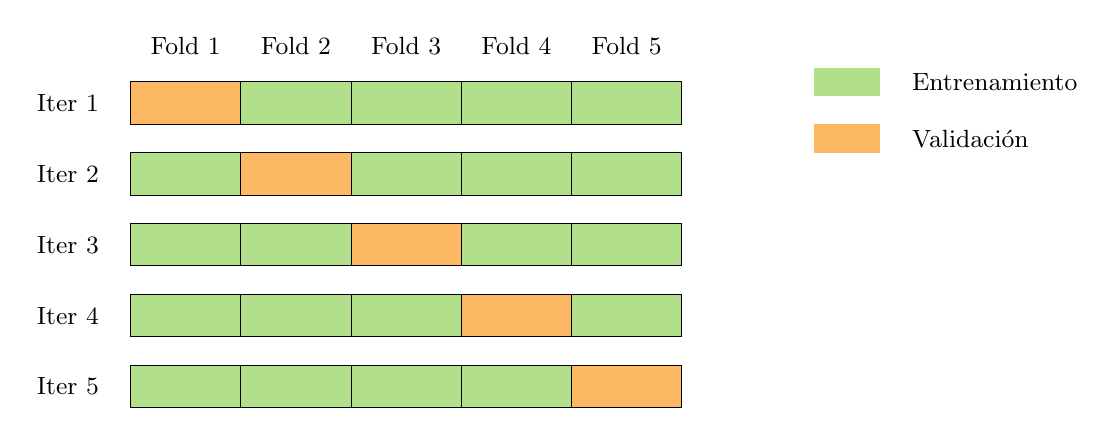
\begin{tikzpicture}[x=1.4cm,y=0.9cm,font=\small]
		%%% Colores
		\definecolor{traincolor}{RGB}{178,223,138} % verde claro
		\definecolor{valcolor}{RGB}{253,184,99}    % naranja claro
		\def\K{5}
		\def\cellh{0.6}

		%%% Cabeceras de columnas (folds)
		\foreach \j [evaluate=\j as \lab using int(\j+1)] in {0,...,4} {
			\node[anchor=south] at (\j+0.5, 0.25) {Fold \lab};
		}

		%%% Cuadrícula: filas = iteraciones, columnas = folds
		\foreach \row [evaluate=\row as \it using int(\row+1)] in {0,...,4} {
			% Etiqueta de fila (iteración/fold de validación)
			\node[anchor=east] at (-0.2, -\row-\cellh/2) {Iter \it};

			\foreach \col in {0,...,4} {
				% Validación: columna que coincide con la fila
				\ifnum\col=\row
				\fill[valcolor] (\col, -\row) rectangle ++(1,-\cellh);
				\else
				\fill[traincolor] (\col, -\row) rectangle ++(1,-\cellh);
				\fi
				\draw (\col, -\row) rectangle ++(1,-\cellh);
			}
		}

		%%% Leyenda
		\begin{scope}[shift={(6.2, -0.2)}]
			\fill[traincolor] (0,0) rectangle ++(0.6,0.4);
			\node[anchor=west] at (0.8,0.2) {Entrenamiento};

			\fill[valcolor] (0,-0.8) rectangle ++(0.6,0.4);
			\node[anchor=west] at (0.8,-0.6) {Validación};
		\end{scope}
	\end{tikzpicture}
	\caption{Esquema de \emph{K-fold Cross Validation} con \(K=5\): en cada iteración, un fold distinto (naranja) se usa para validación y los restantes (verde) para entrenamiento.}
	\label{fig:kfold_cross_validation_ejemplo}
\end{figure}



\subsection{Retropropagación}\label{sec:retropropagacion}

La magia del aprendizaje automático se fundamenta en un algoritmo conocido como retropropagación (\textit{backpropagation}, en inglés). Esta técnica consiste en utilizar una función de coste al final de la red que mida la discrepancia entre el valor inferido y el real. Posteriormente, propagaremos el error desde el final hasta la primera capa de la red, actualizando sistemáticamente todos los parámetros internos que intervienen en la predicción, de forma que en la siguiente iteración hacia adelante (\textit{forward}, en inglés) se reduzca la magnitud del error \cite{dl_fundamentos__casas_roma_2020}.

Existen diferentes funciones de pérdida, todas relacionan la salida esperada $y$ con la predicción del modelo $\hat{y}$. En este trabajo nos centraremos en una de las más básicas y utilizadas en la literatura: el error cuadrático.

\begin{align}\label{f_error:cuadratico}
    E = \frac{1}{2}(\hat{y}-y)^2
\end{align}

A lo largo de la retropropagación, utilizaremos el error calculado por funciones como esta para poder actualizar todos los parámetros. Sin embargo, no todos ellos se actualizarán de la misma forma. Tenemos que ser capaces de discernir qué neuronas estuvieron más implicadas en la decisión de la red, de forma que la magnitud del cambio sea proporcional a la responsabilidad. En el mundo matemático, las herramientas utilizadas para medir la variación de un parámetro respecto de otro es la \textbf{derivada}. Esta es la base del algoritmo utilizado por antonomasia en el entrenamiento de modelos de aprendizaje automático: el descenso del gradiente.

\paragraph{Descenso del Gradiente} \label{sec:descenso_gradiente}

Imaginemos que somos una persona con los ojos vendados en mitad de una montaña. Si quisiéramos descenderla, bastaría con, iterativamente, dar pequeños pasitos en dirección a donde la pendiente sea menor. Básicamente, este es el razonamiento detrás del descenso del gradiente. Siendo la función del error una función continua, podemos calcular la derivada respecto de uno de sus parámetros para estudiar la pendiente y hallar mínimos locales. Eso, en resumen, es lo que hace nuestra red para aprender.

Hagamos un ejemplo con un sistema en $2D$. Supongamos el final de una iteración de nuestro modelo, que nuestra función de coste es el error cuadrático y el valor esperado en la inferencia es 0, nuestra función de coste quedaría $f(x) = \frac{1}{2}(x)^2$. En este punto, siendo la red, tendríamos que calcular cómo varía el error en función del valor de nuestros parámetros. La derivada de nuestra función de coste es $f'(x) = x$. Todo esto se puede escribir en python de forma muy simple utilizando la sintaxis de las expresiones lambda.

\begin{lstlisting}[language=Python,label=code:descenso_grad_2d_1]
	import numpy as np
	f_error = lambda x: 1/2 * (x)**2
	df_error = lambda x: x
\end{lstlisting}

Luego, para representar nuestra función de coste vamos a generar un array de valores que nos permitan ver la gráfica del error centrada. Como la expresión del coste define una parábola con vértice en el $0$, crearemos un vector de $1000$ valores entre el $-1$ y el $1$. Además, seleccionaremos un punto aleatorio de este vector, ya que la inicialización de parámetros es aleatoria.

\begin{lstlisting}[language=Python,label=code:descenso_grad_2d_2]
	data = np.linspace(-1, 1, num=1000)
	rnd_x = np.random.choice(data, 1)
\end{lstlisting}

Es aquí donde entrea en juego nuestro algoritmo de optimización. Vamos a iterar sobre esta función de coste, para cada paso vamos a calcular hacia dónde tiene que moverse nuestro punto para minimizar el error. Para ello, utilizaremos la derivada junto con un factor de cambio que decidimos nosotros. Con él, controlaremos la magnitud del cambio sobre el punto, más tarde ahondaremos en este concepto.

\begin{lstlisting}[language=Python,label=code:descenso_grad_2d_3]
	fig, ax = plt.subplots()
	ax.plot(data, f_error(data), label='f_error', color='black')
	ax.scatter(rnd_x, f_error(rnd_x), color='red', label='inicio')

	change_rate = 0.01
	for _ in range(250):
		slope = df_error(rnd_x)
		rnd_x = rnd_x - slope * change_rate
		step = ax.scatter(rnd_x, f_error(rnd_x), marker='.', color='blue')

	ax.scatter(rnd_x, f_error(rnd_x), color='green', label='final')
\end{lstlisting}

Todas estas iteraciones, nos dan como resultado el descenso de la función de coste definida, bajando su pendiente.

\begin{figure}[hb]
	\centering
	\includegraphics[width=0.6\linewidth]{figures/ejemplos/gradient_descent_2d.png}
	\caption{Descenso del gradiente para el error cuadrático. Cada paso acerca $x$ al mínimo global ($x=0$).}
	\label{fig:descenso_gradiente_2d}
\end{figure}

Aunque es simplista, este ejemplo nos ayuda a hacernos una idea de cómo funciona por dentro la actualización de los parámetros. Claro que, en una red, trabajamos a nivel multidimensional, donde los parámetros son tensores, contenedores $n$-dimensionales. En estos casos la notación se vuelve un poco más verbosa, ya que tenemos que emplear el \textbf{gradiente} \cite{dl_python__chollet_2021}.

Por definición, el gradiente de la función de coste $\nabla E$ es un vector que apunta hacia la dirección de máximo aumento del error. Su magnitud indica la tasa de cambio en esa dirección, es decir, cuanto mayor sea, mayor variación habrá. Por tanto, si buscamos $-\nabla C$, nuestro vector gradiente estará apuntando hacia donde el valor del error se minimiza, que, de hecho, es lo que buscamos para el aprendizaje de la red. Si modificamos un poco el código anterior, podemos realizar un ejemplo en $3D$. En este caso, usando dos vectores, $\vec{x}$ e $\vec{y}$, la función del error la expresaremos con lo que en la literatura se denomina \textit{one-hot encoding}. Esta notación consiste en relacionar las clases de predicción con las posiciones de un vector. Aquellas clases que son correctas se marcan con el valor $1$ en la posición correspondiente, el resto a $0$. Traduciendo el caso anterior, en el que el valor esperado era un $0$. El error se calcularía como $f(x) = \frac{1}{2} ((x-1)^2 + y^2)$.

\begin{lstlisting}[language=Python,label=code:descenso_grad_3d_1]
	f_error = lambda x, y: 1/2 * ((x - 1)**2 + y**2)
	dfdx_error = lambda x: x - 1
	dfdy_error = lambda y: y

	data = np.linspace(-10,10,1000)
	x, y = np.meshgrid(data, data)
	rnd_x = np.random.choice(data, 1)
	rnd_y = np.random.choice(data, 1)

	fig, ax = plt.subplots()
	contour = ax.contourf(x, y, f_error(x,y), levels=10)
	ax.scatter(rnd_x, rnd_y, color='red', label='inicio')

	change_rate = 0.01
	for _ in range(250):
		slope_x = dfdx_error(rnd_x)
		slope_y = dfdy_error(rnd_y)
		rnd_x = rnd_x - slope_x * change_rate
		rnd_y = rnd_y - slope_y * change_rate
		step = ax.scatter(rnd_x, rnd_y, color='blue', marker='.')

	ax.scatter(rnd_x, rnd_y, color='green', label='final')
\end{lstlisting}

Ajustando el resto del código a este formato obtendríamos una representación tridimensional del descenso del gradiente de nuestra función de coste, desde un punto elegido aleatoriamente (punto rojo), paso a paso, hasta el mínimo (global) del error (punto verde).

\begin{figure}[htb]
	\centering
	\includegraphics[width=0.7\linewidth]{figures/ejemplos/gradient_descent_3d.png}
	\caption{Descenso del gradiente en 3D del error cuadrático. Cada paso acerca $(x,y)$ al mínimo global $f(x,y) = 0$.}
	\label{fig:descenso_gradiente_3d}
\end{figure}


A grandes rasgos, en cada iteración el algoritmo de retropropagación se encargará de distribuir ese error a lo largo de todas las conexiones de la red, calculando en cada nodo cómo varía la salida de la red respecto a ese parámetro buscando que la función del error se minimize. Es decir, acabamos de convertir el aprendizaje de la red neuronal en un problema de optimización \cite{dl__goodfellow_2016}.


\paragraph{Actualización de los Parámetros} \label{sec:actualizacion_parametros}

Como hemos visto a lo largo de la implementación del descenso del gradiente, una de las etapas más importantes es la actualización de los parámetros. Gracias a esto, el modelo es capaz de aprender por cuenta propia, ajustándose automáticamente para ser capaz de inferir con precisión. Comúnmente, a la hora de actualizar los parámetros se utiliza lo que se denomina la \textbf{regla delta} en la literatura. Esto no es más que una formalidad para referirse al incremento o el decremento del valor de los parámetros.

\begin{equation}\label{regla_delta}
	\Delta x = \eta \frac{dE}{dx} \rightarrow x = x - \frac{dE}{dx}
\end{equation}

En esta expresión redescubrimos un factor muy importante en la actualización de los pesos. Previamente, en el descenso del gradiente, regulamos la magnitud del cambio calculado en la derivada con un ratio de cambio. Este ratio de cambio expresa la "velocidad" a la que queremos que nuestro modelo aprenda. En la literatura se conoce como \textbf{tasa de aprendizaje} y en función de su valor, podemos provocar que el modelo aprenda tan lento que nunca llegue a adquirir todas las características del problema, pudiendo incluso estancarse en mínimos locales; o por el contrario, si la tasa es muy grande, el modelo difícilmente encuentrará el mínimo en el error. La elección de la tasa de aprendizaje determina la velocidad y la estabilidad del entrenamiento. Un valor óptimo permitirá a la red descender suavemente hacia configuraciones de error mínimo \cite{dl_python__chollet_2021, dl_fundamentos__casas_roma_2020, dl__goodfellow_2016}.

Con este ejemplo hemos podido comprender mejor cómo funciona la optimización de parámetros en una red monocapa. Pero ¿qué ocurre cuando tenemos más de una capa? El descenso del gradiente es una técnica que nos permite saber cómo serán las variaciones del error en función de los parámetros de la capa directamente anterior a la salida. Es decir, al utilizar redes multicapa sólo podríamos afinar los parámetros de las neuronas de la penúltima capa de la red. Es aquí donde, la regla de la cadena, entra en juego, permitiéndonos calcular fácilmente el gradiente de arquitecturas complejas \cite{dl_python__chollet_2021}.


\paragraph{La Regla de la Cadena} \label{sec:regla_cadena}

Recapitulando un poco, hemos logrado adquirir las herramientas necesarias para calcular cómo corregir el error de predicción de nuestro modelo. Sin embargo, nuestros modelos son complejas estructuras de cálculo, pareciese que el cálculo final del error no tuviese nada que ver con aquella entrada en la primera capa. ¿O sí? Cierto es que nuestros modelos son complejas redes de nodos interconectados, donde cada salida depende de una serie de operaciones intermedias. Para poder ajustar los parámetros desde la última capa hasta la primera necesitamos una manera sistemática de propagar esas derivadas hacia atrás a lo largo de la red.

Aquí entra en juego la regla de la cadena, una herramienta matemática que nos permite descomponer la derivada de una función en términos de derivadas parciales más simples. En otras palabras, la regla de la cadena actúa como un mecanismo de transmisión: el gradiente fluye desde la salida hasta las entradas atravesando cada operación que conecta ambos extremos. En la literatura, se utilizan una serie de expresiones matemáticas \footnote{Consultar \ref{anexo:retropropagacion}.}. No obstante, este trabajo pretende arrojar un pequeño haz de luz e intuición. Por tanto, nos centraremos en la idea sobre la que se construyeron los modelos matemáticos.

Para entenderlo de forma intuitiva, consideremos un ejemplo sencillo $f(x,y,z) = (x+y)z$, que podemos simplificar todavía más como $q=(x+y)$ y $f=qz$. En la figura \ref{fig:forward_pass_diagrama} se muestra el grafo que desglosa las operaciones para $f(2,3,4)$.

\begin{figure}[ht]
	\centering
	\includegraphics[width=0.6\linewidth]{figures/ejemplos/forward_diagram.png}
	\caption{Diagrama de la función $f(x,y,z)=(x+y)z$, para $(x,y,z)=(2,3,4)$.}
	\label{fig:forward_pass_diagrama}
\end{figure}

Este diagrama, en esencia, representa lo que ocurre en una red al hacer \textit{forward}. Ahora, queremos calcular la responsabilidad de cada entrada dentro de la operación para, en caso de querer corregir los valores, saber la magnitud con la que actualizaremos cada uno. Es decir, tenemos que calcular las derivadas parciales de $f$ respecto de cada entrada: $\frac{\partial f}{\partial x}$, $\frac{\partial f}{\partial y}$ y $\frac{\partial f}{\partial z}$. Para ello, aplicaremos la regla de la cadena de las derivadas. Esta nos dice que podemos descomponer la derivada de una función en términos más simples. En nuestro caso, utilizaremos la expresión $f=qz$ como paso intermedio para calcular las derivadas parciales respecto de $x$ e $y$.

\begin{equation}
	\frac{\partial f}{\partial x} = \frac{\partial f}{\partial q} \frac{\partial q}{\partial x} \qquad
	\frac{\partial f}{\partial y} = \frac{\partial f}{\partial q} \frac{\partial q}{\partial y}
\end{equation}

Para $z$ no tenemos el mismo inconveniente, ya que en la expresión $f=qz$ existe una relación directa entre la función y la variable. Ahora sí, podemos calcular paso a paso las derivadas parciales por la regla de la cadena:

\begin{figure}[h!]
	\centering
	\includegraphics[width=0.6\linewidth]{figures/ejemplos/backward_diagram.png}
	\label{fig:backward_diagrama}
	\caption{Diagrama de regla de la cadena de la función $f(x,y,z)=(x+y)z$, para $(x,y,z)=(2,3,1)$.}
\end{figure}

En resumen, la retropropagación permite trasladar la información del error desde la salida de la red hasta sus capas más profundas mediante la aplicación sistemática de la regla de la cadena. Gracias a este mecanismo, cada parámetro recibe una corrección proporcional a su contribución en la predicción final. Este procedimiento convierte a la retropropagación en el motor principal del aprendizaje en redes neuronales: a través de sucesivas iteraciones de propagación hacia adelante, cálculo de error y propagación hacia atrás, el modelo ajusta sus parámetros internos hasta capturar patrones útiles en los datos.

De este modo, lo que en apariencia es un entramado complejo de nodos y conexiones, se convierte en un sistema entrenable y optimizable. Esta combinación de cálculo diferencial y optimización numérica constituye la base matemática sobre la que se sustentan las arquitecturas modernas de aprendizaje profundo.


\subsection{Generalización y Regularización}

Hasta el momento, hemos abordado el aprendizaje de una red neuronal como un problema de optimización, con el propósito principal de entrenar modelos que no solo funcionen bien con los datos utilizados durante el entrenamiento, sino que también sean capaces de realizar predicciones precisas en datos nuevos. Esta capacidad de desempeñarse correctamente en situaciones no vistas previamente se conoce como \textit{generalización} \cite{dl__goodfellow_2016}. En esencia, buscamos desarrollar modelos que identifiquen patrones útiles y aplicables a distintos contextos, evitando simplemente memorizar los ejemplos específicos del conjunto de entrenamiento.

\paragraph{Problemas comunes en el entrenamiento}
De acuerdo con \citeauthor{dl__goodfellow_2016}, la capacidad de un modelo para generalizar correctamente depende tanto de su habilidad para minimizar el error en los datos de entrenamiento como de su eficacia al enfrentarse a las diferencias entre los conjuntos de entrenamiento y prueba. En este contexto, se identifican principalmente los siguientes problemas:

\begin{itemize}
	\item \textbf{Sobreajuste}: ocurre cuando la red neuronal memoriza detalles irrelevantes del conjunto de entrenamiento en lugar de aprender patrones significativos. El resultado es un rendimiento deficiente en datos nuevos.
	\item \textbf{Subajuste}: aparece cuando el modelo es demasiado simple para capturar la complejidad de los datos, lo que impide alcanzar un buen desempeño incluso en el propio conjunto de entrenamiento.
	\item \textbf{Alta varianza y sesgo}: relacionados respectivamente con modelos excesivamente complejos (varianza elevada) o excesivamente simples (alto sesgo).
\end{itemize}

Para mitigar estas situaciones, existen diversas técnicas que actúan directamente sobre los parámetros del modelo durante el entrenamiento, conocidas como regularización, entre las más utilizadas se encuentran la L1 y L2, el dropout y la normalización de los batches.

\textbf{Regularización L1.} Consiste en añadir un término proporcional a la suma de los valores absolutos de los pesos en la función de pérdida:

\begin{equation}
	\mathcal{L}_{total} = \mathcal{L}_{original} + \lambda \sum_{i} |w_i|
	\label{eq:l1_reg}
\end{equation}

Este mecanismo promueve la \textit{esparsidad} en los parámetros, forzando a que muchos de ellos tomen valor cero. De este modo, el modelo tiende a ser más simple y puede realizar una selección implícita de características relevantes.

\textbf{Regularización L2.} También denominada \textit{weight decay}, esta técnica penaliza la magnitud cuadrática de los pesos:

\begin{equation}
	\mathcal{L}_{total} = \mathcal{L}_{original} + \lambda \sum_{i} w_i^2
	\label{eq:l2_reg}
\end{equation}

A diferencia de L1, no fuerza explícitamente pesos nulos, pero sí tiende a mantenerlos pequeños. Esto contribuye a estabilizar el entrenamiento y mejorar la capacidad de generalización al evitar que el modelo dependa en exceso de ciertos parámetros.

\textbf{Dropout.} Es una técnica estocástica que consiste en "desactivar" de forma aleatoria un subconjunto de neuronas durante cada paso del entrenamiento, el tamaño de ese subconjunto se suele configurar entre un $0.2$ y un $0.5$ del total de neuronas de la capa. De esta forma, la red no puede depender excesivamente de neuronas concretas y se ve obligada a explorar otros caminos dentro de la red, volviéndose más robusta. Cuando no se entrena, todas las neuronas se activan y sus salidas se escalan con el factor de dropout para compensar el efecto del entrenamiento \cite{dl_python__chollet_2021}.

\begin{figure}[h]
	\centering
	\begin{tikzpicture}[>=Latex, every node/.style={font=\small}]
		% Parámetros
		\def\nin{5}   % número de neuronas en la capa l
		\def\nout{4}  % número de neuronas en la capa l+1
		\def\dy{1.2}  % separación vertical entre neuronas
		\def\dx{4.0}  % separación horizontal entre capas

		% Capa 1 (entradas)
		\foreach \i in {1,...,\nin}{
			\node[circle, draw, minimum size=8mm] (I\i) at (0,-\i*\dy) {};
		}
		\node[above=2mm of I1] {Capa $l$};

		% Coordenada y del centro de la primera capa
		\pgfmathsetmacro{\yin}{-(\nin+1)/2 * \dy}

		% Coordenada y del centro de la segunda capa
		\pgfmathsetmacro{\yout}{-(\nout+1)/2 * \dy}

		% Capa 2 (salidas), centrada verticalmente respecto a la capa 1
		\foreach \j in {1,...,\nout}{
			\node[circle, draw, minimum size=8mm] (O\j) at (\dx,{\yin+\yout + \j*\dy}) {};
		}
		\node[above=8mm of O4] {Capa $l+1$};

		% Conexiones por defecto
		\foreach \i in {1,...,\nin}{
			\foreach \j in {1,...,\nout}{
				\draw[gray!60] (I\i) -- (O\j);
			}
		}

		% Resaltar dos neuronas apagadas en capa l
		\node[circle, draw, minimum size=8mm, fill=gray!30] at (I2.center) {};
		\node at (I2.center) {\textcolor{red}{\Large$\times$}};

		\node[circle, draw, minimum size=8mm, fill=gray!30] at (I4.center) {};
		\node at (I4.center) {\textcolor{red}{\Large$\times$}};

		% Dibujar conexiones activas más fuertes desde las otras neuronas
		\foreach \j in {1,...,\nout}{
			\draw[->, thick, blue] (I1) -- (O\j);
			\draw[->, thick, blue] (I3) -- (O\j);
			\draw[->, thick, blue] (I5) -- (O\j);
		}
	\end{tikzpicture}
	\caption{Ilustración del dropout: algunas neuronas (en gris con aspa) se desactivan de forma aleatoria durante el entrenamiento, forzando a la red a no depender de unidades específicas.}
	\label{fig:dropout}
\end{figure}



\textbf{Batch Normalization.} Aplica una transformación que mantiene la media de la salida a 0 y la desviación estándar a 1. No funciona igual durante el entrenamiento que durante la inferencia. Durante el entrenamiento, utiliza la media y la desviación estándar del batch para normalizar los datos de entrada. Durante las inferencias, el modelo utiliza un promedio móvil de la media y la desviación estándar de los batches que vió en el entrenamiento. Esta técnica, facilita la retropropagación de los gradientes del modelo, lo cual ayuda en modelos profundos \cite{dl__goodfellow_2016}.

En conjunto, estas técnicas permiten controlar la complejidad del modelo y mitigar el sobreajuste, contribuyendo a un mejor equilibrio entre rendimiento en entrenamiento y capacidad de generalización en datos no vistos.

\section{Limitaciones de las Redes Neuronales Tradicionales}\label{sec:limitaciones_rn}

Las redes neuronales densamente conectadas, aunque son efectivas en tareas de aprendizaje general, presentan desafíos al aplicarse a multidimensionales, como las imágenes.

Una de sus principales limitaciones es su incapacidad para aprovechar la estructura espacial. Por ejemplo, en imágenes, trata cada píxel como una entrada independiente, ignorando las relaciones de proximidad entre píxeles adyacentes, fundamental para identificar patrones locales como bordes, texturas o formas.

\begin{figure}[h]
	\centering
	\includegraphics[width=0.7\linewidth]{figures/ejemplos/imagen_a_red_neuronal.png}
	\caption{Aplanado de una imagen para servir de entrada a una red neuronal.}
	\label{fig:aplanado_imagen_red_neuronal}
\end{figure}

Adicionalmente, esta condición provoca lo que se conoce como \textit{redundancia en el aprendizaje de características}, donde cada neurona debe aprender pesos específicos para detectar una característica en una posición particular, como por ejemplo la neurona $a_{3}^{1}$ de la figura \ref{fig:aplanado_imagen_red_neuronal}, incluso si dicha característica ha aparecido en otra región de la imagen, limitando su generalización.

Por otra parte, intentar modelar problemas que involucren imágenes de gran
tamaño (por ej. 100x100 píxeles) puede convertirse en un reto de escalabilidad en el que los parámetros
crezcan exponencialmente. Una capa densa con 1000 neuronas requeriría millones
de pesos, lo que conlleva un alto coste computacional, riesgo de overfitting y
un alto consumo de memoria.

Con la intención de sobrepasar dichas limitaciones, las redes convolucionales introducen mecanismos específicos adaptados a datos visuales. Mediante operaciones de \textbf{convolución}, que aplican filtros locales que trabajan con \textit{ventanas} en la imagen, permitiendo al modelo preservar la estructura bidimensional de la entrada y aprender patrones espaciales jerárquicamente.


    \chapter{Redes Neuronales Convolucionales}\label{cap:red_neuronal_convolucional}

A raíz de las limitaciones encontradas en las redes neuronales tradicionales, el mundo de la visión por computador se vio "forzado" a buscar otras técnicas más especializadas. No sólo desde el punto de vista de la precisión de los modelos, sino también, del rendimiento. Como hemos comentado en secciones anteriores, los modelos de inferencia tradicional necesitan una gran cantidad de recursos para poder trabajar con información espacial, factor que en muchas ocasiones se convierte en limitante.

La necesidad de un enfoque más eficiente dio lugar al desarrollo de las Redes Neuronales Convolucionales, que basan su funcionamiento en la operación de la convolución. Esta herramienta matemática permite extraer características de conjuntos de datos $n$-dimensionales guardando las relaciones espaciales entre los nodos, lo que la convierte en la candidata perfecta para superar las limitaciones presentadas por arquitecturas tradicionales. Estas técnicas permiten a los modelos de convolución \textbf{reconocer patrones locales} y elementos como bordes, texturas o contornos y sus relaciones entre diferentes regiones de una imagen de una forma más natural, como hacemos los seres humanos para reconocer objetos como pelotas, coches, animales, etc.

\begin{figure}[ht]
	\centering
	\includegraphics[width=1\linewidth]{figures/ejemplos/LeNet-5_architecture.png}
	\caption{Arquitectura LeNet-5 \cite{zhang2023dive}.}
	\label{img:lenet-5}
\end{figure}

Por otro lado, la arquitectura convolucional nos permite simplificar mucho la cantidad de parámetros que debe gestionar el modelo para llevar a cabo su tarea, en comparación con modelos tradicionales, como los perceptrones multicapa (MLP, en inglés), donde fácilmente podemos llegar a acumular centenas de miles de parámetros de conexiones entre cada par de neuronas. Esto es gracias a la \textbf{compartición de pesos} en las capas de convolución, que utilizan filtros (cuyos valores son parámetros de la red) que se aplican repetidamente sobre diferentes regiones de la imagen, lo que nos permite, no sólo encontrar patrones similares en diferentes regiones, sino que también reducir drásticamente el consumo de memoria, mejorar la eficiencia y la generalización del modelo.

Otro aspecto fundamental de las redes convolucionales es su capacidad para realizar una \textbf{descomposición jerárquica} de las características presentes en los datos de entrada. En las capas iniciales, los filtros tienden a detectar patrones muy simples, como bordes horizontales, verticales o diagonales. Conforme se avanza en profundidad, las siguientes capas combinan estas representaciones elementales para formar descriptores más complejos, como esquinas, texturas o regiones específicas de un objeto. Finalmente, en las capas más profundas, la red es capaz de representar estructuras de alto nivel a partir de la composición de las características aprendidas previamente. Este proceso refleja, en cierto modo, la manera en que el sistema visual humano descompone la información visual en niveles de complejidad creciente \cite{dl_python__chollet_2021, nn_dl__michael_nielsen_2015, dl__goodfellow_2016}.

Algunos de los hitos más relevantes en modelos convolucionales fueron la arquitectura \textit{LeNet-5}, propuesta por \citeauthor{lecun-98} en \citeyear{lecun-98}, diseñada para el reconocimiento de dígitos y letras manuscritas. Este modelo mostró por primera vez el potencial de las convoluciones para extraer características jerárquicas de las imágenes de forma automática, tanto que esta tecnología acabó implementándose en las máquinas bancarias ATM para leer cheques \cite{lecun-98}.

\begin{figure}[ht]
	\centering
	\includegraphics[width=1\linewidth]{figures/ejemplos/AlexNet_Original_block_diagram.png}
	\caption{Arquitectura AlexNet \cite{Krizhevsky2012ImageNetCW}.}
	\label{img:alexnet}
\end{figure}


Más tarde, por el año 2012, el interés en las redes convolucionales incrementó cuando \textit{AlexNet}, un modelo de clasificación convolucional logró una mejora drástica en el ILSVRC (\textit{ImageNet Large Scale Visual Recognition Challenge}), una competición mundialmente conocida por evaluar el rendimiento y desempeño de arquitecturas de detección de objetos y clasificación de imágenes de gran tamaño \cite{imagenet-web}. Este novedoso modelo consiguió reducir a la mitad el error de clasificación respecto al mejor sistema hasta ese momento \cite{Krizhevsky2012ImageNetCW}. Este resultado marcó el inicio de la adopción masiva de los modelos convolucionales y consolidó su papel como modelo de referencia en visión por computador.

Actualmente, las redes convolucionales tienen una amplia variedad de aplicaciones prácticas: reconocimiento facial en sistemas de seguridad, detección de objetos en conducción autónoma, análisis médico de imágenes como radiografías o resonancias magnéticas, clasificación de imágenes por satélite o incluso el procesamiento de vídeo en tiempo real \cite{nn_fundamentals__thakur_2021, rna_fundamentos__hilera_2021, conv_nn_face_recog__chowanda_2019}.



\section{Arquitectura de una Red Neuronal Convolucional}\label{sec:arquitectura_cnn}

Las redes convolucionales son famosas por su arquitectura que, a menudo, recuerda a la forma de un embudo. Se desglosa en una serie de capas con orden concreto. Cada una de ellas está especializada en tareas concretas para obtener cierta información de las entradas. Esta configuración permite a la red aprender representaciones progresivamente más abstractas y complejas.


\paragraph{Capa convolucional}

Además de darle el nombre a la arquitectura, es en esta capa en la que reside la clave del éxito de los modelos convolucionales. Como mencionamos anteriormente, la principal diferencia con los modelos tradicionales se encontraba en la forma en la que se interpreta y relaciona la información espacial de los datos de entrada a la red. Esto es posible gracias a la operación de convolución que llevan a cabo en su interior.

La \textbf{convolución} es un operador matemático que transforma dos funciones $f$ y $g$ en una tercera función que, de cierta forma, representa la superposición de $f$ y $g$ a lo largo del tiempo \cite{dl__goodfellow_2016}. Intuitivamente, puede entenderse como una operación en la que una de las funciones se "desliza" sobre la otra, midiendo en cada posición el grado de similitud entre ambas.

\begin{figure}[ht]
	\centering
	\includegraphics[width=0.7\linewidth]{figures/ejemplos/convolucion_f_g_discretas.png}
	\caption{Convolución discreta entre $f = [0,0,1,1,0,0]$ y filtro de detección de bordes $g = [-1,0,1]$.}
	\label{fig:convolucion_f_g_discreta}
\end{figure}

En las capas convolucionales, consiste en desplazar pequeñas matrices denominanadas \textit{filtros} o \textit{kernels} a lo largo de la imagen de entrada a la capa y realizar una serie de cálculos entre los valores de nuestra matriz y los de la entrada que nos ayudarán a detectar características importantes \cite{nn_dl__michael_nielsen_2015}.

\begin{figure}[ht]
	\centering
	\includegraphics[width=1\linewidth]{figures/ejemplos/convolucion_sobel.png}
	\caption{Convolución con filtro de Sobel en ejes ${x,y}$ para detectar bordes.}
	\label{fig:convolucion_sobel}
\end{figure}

Por ejemplo, en la figura \ref{fig:convolucion_sobel}, hemos aplicado el filtro de Sobel, kernel conocido por su capacidad para localizar bordes verticales y horizontales, para localizar las regiones de la imagen en las que podemos encontrar dichas características. Cada una de estas detecciones puede ser una de las salidas de un filtro de las primeras capas de convolución de la red. A medida que avanza la información por las diferentes capas convolucionales, se irán detectando más características, consiguiendo que la red sea capaz de captar detalles más concretos, como curvas, o contornos. Claro que, a diferencia de este ejemplo, en una capa convolucional generalmente obtenemos muchas más salidas, concretamente, tantas como filtros pasemos, por ejemplo, la salida de pasar una imagen de $28\times28$ por una capa convolucional con 32 filtros de $3\times3$ nos devuelve $32$ imágenes de $26\times26$ (fig. \ref{fig:conv1_salidas}).

\begin{figure}[ht]
	\centering
	\includegraphics[width=1\linewidth]{figures/ejemplos/conv1_salidas.png}
	\caption{Salida de una capa convolucional con $32$ filtros de $3\times3$.}
	\label{fig:conv1_salidas}
\end{figure}


\paragraph{Capa de activación}

Generalmente, las operaciones matriciales que estamos realizando sobre las entradas pueden descomponerse como una combinación lineal de la forma $W_2(W_1x)=(W_2W_1)x$. Esto aporta un inconveniente muy grande, ya que la complejidad de nuestra arquitectura se simplificaría en una combinación lineal de las entradas con los parámetros de la red, provocando que nuestro modelo no sea capaz de aprender patrones más complejos. Para corregir esta laguna en nuestra arquitectura convolucional, introducimos una herramienta utilizada de igual forma en los modelos tradicionales: las funciones de activación. Concretamente, en este trabajo se utiliza la ya mencionada ReLU (\ref{sec:relu}), definida como $f(x) = \max(0, x)$. Donde, para $x > 0$, el comportamiento es lineal, mientras que para $x \le 0$, la salida es constante, consiguiendo de esta forma introducir no linealidad en el modelo \cite{dl_fundamentos__casas_roma_2020, dl__goodfellow_2016}.

\begin{figure}[h]
	\centering
	\includegraphics[width=0.6\linewidth]{figures/ejemplos/no_linealidad_relu.png}
	\caption{Comparación entre una red lineal y una con activación ReLU. La introducción de no linealidad permite modelar funciones más complejas.}
	\label{fig:relu_network}
\end{figure}


\paragraph{Capa de pooling}

Anteriormente, mencionamos que los modelos convolucionales tienen la capacidad de hacer una descomposición jerárquica de los datos de entrada. Las capas convolucionales, junto con las de activación, son las encargadas de extraer las características de nuestras imágenes. Sin embargo, nos falta un hilo conector muy importante para terminar de preparar esa información para las capas posteriores del modelo. Es aquí donde entran en juego las capas de pooling. La operación de pooling se refiere a una transformación cuya finalidad es reducir la dimensionalidad de la entrada. Para ello, normalmente se aplica una operación estadística el máximo, la media, o incluso la normalización L2, entre los valores seleccionados por una ventana de tamaño $n \times m$.

\begin{figure}[ht]
	\centering
	\includegraphics[width=0.8\linewidth]{figures/ejemplos/pooling_2d.png}
	\caption{Operación de Max Pooling con una ventana de $2\times2$.}
	\label{fig:pooling_2d}
\end{figure}

Además, las operaciones de pooling ayudan a que el modelo sea capaz de extraer y reconocer patrones sin importar pequeñas modificaciones en las entradas. Es decir, aplicando pooling introducimos invarianza ante traslaciones locales de las características, volviendo nuestra arquitectura más robusta. Algunos de los filtros de pooling más utilizados son el \textit{Max Pooling}, o el \textit{Avg Pooling} \cite{dl__goodfellow_2016}.

En la literatura y en las arquitecturas actuales, lo más común es encontrarnos la tríada de capas convolucional-relu-pooling, ya que esta configuración ayuda a dar robustez al modelo y permite construir estructuras más complejas y profundas sin que el rendimiento de la red se vea agravado.

\paragraph{Capa completamente conexa}

Llegamos a la parte final de nuestra arquitectura. Después de haber extraído todas las características aprovechando nuestros operadores espaciales, nuestra red introduce toda esa información en un conjunto de capas completamente conexas, similares a las de modelos tradicionales, donde se calcularán las relaciones entre los patrones extraídos y las clases sobre las que tenemos que predecir. Para ello, la salida de la última capa convolucional se suele aplanar para servir de entrada a la primera capa densa del modelo \cite{nn_dl__michael_nielsen_2015}.

Intuitivamente, podemos pensar en la arquitectura de una red convolucional como dos partes especializadas. La primera, que se encarga de extraer características útiles para identificar a las diferentes clases, lo cual tiene un coste computacional muy alto empleando arquitecturas tradicionales. Y la segunda, que se encarga de procesar esa información "masticada" previamente por el bloque convolucional, siendo capaz de inferir la pertenencia a cada clase.



\section{Funcionamiento Interno: Filtrado, Stride y Padding}\label{sec:funcionamiento_interno_cnn}

Como hemos ido viendo a lo largo de las secciones anteriores, las redes convolucionales se basan en la operación de convolución, donde un filtro se desplaza sobre la entrada y aplica una transformación con la que obtiene características concretas. Además, cada uno de estos filtros puede transformar dimensionalmente la entrada que reciben, reduciéndola, estirándola, etc. Por ello, a la hora de entrenar nuestros modelos, las dimensiones de los filtros, así como la forma en que los desplazamos por las entradas son hiperparámetros\footnote{Los hiperparámetros son parámetros de un modelo o del proceso de entrenamiento que \textbf{no se aprenden automáticamente} durante el entrenamiento, sino que los definimos nosotros previamente. Por ejemplo: el número de capas, la tasa de aprendizaje o el número de filtros a utilizar \cite{dl__goodfellow_2016}.} de configuración muy importantes, que pueden afectar directamente a la capacidad de la red para aprender y a la eficiencia computacional.

\paragraph{Dimensiones del filtro}

El tamaño de nuestros filtros es un factor clave dentro del aprendizaje. Filtros pequeños ($2\times2$ o $3\times3$) capturan detalles locales de la escena, algo así como si mirásemos desde un microscopio. Por otro lado, los filtros grandes ($7\times7$ o $11\times11$) permiten captar detalles más generales, con el inconveniente de requerir un mayor número de parámetros. Es decir, la dimensión que seleccionemos, no sólo va a determinar la forma en la que nuestro modelo aprenda, sino que va a afectar directamente en nuestro rendimiento computacional.

Además, desplazar un filtro de una determinada dimensión puede conllevar modificar la extensión de nuestra entrada en todos sus ejes. Es el caso de la figura \ref{fig:stride_avg_pooling} al pasar un filtro de tamaño $2\times2$ a nuestra entrada de $4\times4$, reducimos sus dimensiones a $3\times3$.

\paragraph{Stride}

Define el número de píxeles que avanza el filtro en cada paso. Con $\text{stride}=1$, el filtro se desplaza píxel a píxel, produciendo una salida de tamaño similar a la entrada. Con $\text{stride} \ge 2$, avanza dando saltos de $n$ píxeles tal que $n \ge 2$, reduciendo la dimensionalidad del resultado. A mayores valores, el stride provoca que la inferencia se haga muy rápido, con el inconveniente de que puede significar perder de información importante en las entradas.

\begin{figure}[h]
	\centering
	\includegraphics[width=0.65\linewidth]{figures/ejemplos/stride_avg_pooling.png}
	\caption{Ejemplo de average pooling con stride $= 1$ y stride $= 2$.}
	\label{fig:stride_avg_pooling}
\end{figure}

\paragraph{Padding}

En una convolución, al aplicar un kernel sobre una imagen, los píxeles situados en los bordes se "visitan" menos porque el filtro no puede extenderse más allá de los límites de la imagen. Este hiperparámetro nos permite configurar filas y columnas extra de relleno, normalmente a $0$, alrededor de la imagen para preservar la información de los bordes. Además, ajustando bien el padding podemos mantener el tamaño de entrada. Por ejemplo, una imagen de $4 \times 4$ con un filtro de $3 \times 3$ devuelve una imagen de $2 \times 2$. Con el padding adecuado, en este caso $\text{padding}=1$, puede mantenerse en $4 \times 4$. Es decir, el padding nos permite controlar el equilibrio entre reducir la dimensionalidad y preservar la información.

\begin{figure}[h]
	\centering
	\includegraphics[width=0.8\linewidth]{figures/ejemplos/padding_avg_pooling.png}
	\caption{Ejemplo de average pooling con $\textbf{padding}=1$.}
	\label{fig:padding_avg_pooling}
\end{figure}

De esta forma, diseñar las capas convolucionales de nuestra red se convierte en un meticuloso trabajo artesanal para ajustar estos hiperparámetros de modo que la potencia del modelo y su eficiencia computacional estén equilibrados \cite{dl_python__chollet_2021, dl_fundamentos__casas_roma_2020, dl__goodfellow_2016}.



\section{Aprendizaje y Optimización de Filtros}\label{sec:ajuste_parametros_cnn}

El verdadero poder de las redes convolucionales reside en su capacidad de aprender de forma automática los filtros adecuados para extraer las características específicas que le permitan discernir adecuadamente entre las diferentes clases. Aquí entra en juego nuestro algoritmo de aprendizaje por antonomasia, la retropropagación. Al igual que los modelos tradicionales ajustan los pesos sus conexiones en base al error obtenido, los modelos convolucionales aprovechan estas iteraciones para afinar sus filtros.

\paragraph{Retropropagación en las capas convolucionales}

El aprendizaje de los filtros sigue el mismo principio que en modelos tradicionales: los pesos (en este caso, los valores de los kernels) se inicializan aleatoriamente y se ajustan iterativamente mediante el algoritmo de retropropagación del error (\ref{sec:retropropagacion}).
La retropropagación permite calcular el gradiente de la función de pérdida con respecto a cada parámetro de la red, propagando los errores desde la capa de salida hacia las capas anteriores. Este gradiente se usa para actualizar los pesos en la dirección que se minimiza la pérdida.

\paragraph{Optimización}

Para actualizar los parámetros, se utilizan algoritmos de optimización basados en el descenso del gradiente \ref{sec:descenso_gradiente}. El descenso de gradiente estocástico (SGD) es la técnica clásica, donde los parámetros se actualizan tras cada minibatch de datos.
En la práctica, se emplean variantes más sofisticadas como Adam, RMSProp o Momentum, que aceleran la convergencia y mejoran la estabilidad del entrenamiento \cite{dl_python__chollet_2021}.



\subsection{Visualización de activaciones}

{\color{red} AÑADIR IMÁGENES DE LAS ACTIVACIONES}

Una forma de comprender mejor cómo aprende nuestro modelo, y así, lograr un mejor ajuste de hiperparámetros o detectar posibles problemas en el entrenamiento, es mediante una técnica conocida como la visualización de activaciones. Consiste en inspeccionar los mapas de características que produce cada filtro en distintas capas de la red al procesar una imagen.
En las primeras capas suelen observarse activaciones asociadas a bordes y texturas simples, mientras que en capas más profundas aparecen representaciones cada vez más abstractas, como formas u objetos parciales \cite{dl_python__chollet_2021}.



    \chapter{Herramientas de Visualización}\label{cap:herramientas_visualizacion}

En el mundo científico, a menudo utilizamos el término \textbf{caja negra} para hacer referencia a sistemas complejos que producen una salida coherente a partir de una entrada dada, pero cuyo funcionamiento interno es difícilmente interpretable o accesible para el observador, como en el caso de las redes neuronales profundas, donde el conocimiento de la red está distribuido en pesos y activaciones de múltiples capas interconectadas.

Por ello, a lo largo del tiempo, se han desarrollado diferentes métodos que nos ayudan a analizar qué ocurre dentro de los modelos, lo que nos permite entender por qué ciertos patrones arquitectónicos funcionan mejor que otros dependiendo del problema, o incluso a ajustar con mayor precisión y de forma más acertada los hiperparámetros del modelo \cite{dl_python__chollet_2021, dl__goodfellow_2016}.

En esta sección se hablará sobre los métodos de visualización más populares en la literatura de redes profundas. Los dividiremos en dos grupos: los que utilizan información del \textit{forward} de la red, como los mapas de características y las activaciones neuronales; y los que se basan en las operaciones con el gradiente en la retropropagación para construir las salidas, como los mapas de saliencia o el Grad-CAM.

\section{Mapas de Características y Activaciones}

Empezando por el más simple, los mapas de características (del inglés, \textit{feature maps}) son las salidas obtenidas al realizar la convolución de la imagen de entrada con cada uno de los filtros de las capas convolucionales de la red. Cada filtro actúa como un \textbf{detector de patrones locales en la entrada}.

\begin{figure}[htb]
	\centering
	\includegraphics[width=0.7\linewidth]{figures/ejemplos/mapa_caracterisicas_con_kernel.png}
	\caption{Mapa de características obtenido al pasar el kernel K2 de una capa convolucional por una imagen de entrada.}
	\label{fig:mapa_caracterisitcas_kernel_k2}
\end{figure}

En las primeras capas suelen aparecer activaciones que corresponden a \textbf{bordes}, \textbf{esquinas} o \textbf{texturas simples}. Conforme nos adentramos en la red, las activaciones reflejan representaciones cada vez más abstractas: desde contornos y formas como curvas o ángulos, hasta estructuras más complejas, como objetos, en las últimas capas \cite{nn_dl__michael_nielsen_2015}.

Visualizando los mapas de características asociados a una imagen concreta podemos averiguar qué filtros destacan regiones importantes de la imagen, haciéndonos entender fácilmente cómo la red interpreta la información. Por ejemplo, en la figura \ref{fig:convolucion_sobel}, el filtro de sobel aplicado sobre el eje de abscisas de una imagen revela bordes horizontales. Mientras que, sobel aplicado en el eje de ordenadas de una imagen revela bordes verticales.

\paragraph{Activaciones Neuronales}

Mediante la comparación de las activaciones entre diferentes ejemplos, se puede analizar la consistencia de los patrones aprendidos. Si varias imágenes que pertenecen a la misma clase provocan respuestas similares en ciertas neuronas, puede inferirse que dichos nodos codifican características relevantes para esa categoría. Por ejemplo, al introducir un dígito del conjunto MNIST, una neurona de una capa intermedia puede activarse principalmente en presencia de trazos verticales, mientras que otra responde mejor a curvas cerradas \cite{nn_dl__michael_nielsen_2015}.

Estas visualizaciones son especialmente útiles durante la fase de desarrollo, ya que permiten detectar errores en el entrenamiento y ajustar la arquitectura o los hiperparámetros de forma más acertada.

\section{Métodos Basados en el Gradiente}

Los métodos basados en el gradiente ofrecen una forma más precisa de entender qué características concretas de la entrada contribuyen a la decisión final del modelo. A diferencia de las visualizaciones de las activaciones, que muestran qué detecta cada capa, estas técnicas indican qué parte de la entrada causó la activación.

\paragraph{Mapas de Saliencia (Saliency Maps)}
Consisten en calcular la derivada de la salida (por ejemplo, la probabilidad de una clase) con respecto a los píxeles de la entrada (la imagen), obteniendo un mapa de calor cuyos valores de mayor magnitud indican los píxeles más relevantes para la predicción \cite{visualizing__simonyan__2014}. Matemáticamente, consiste en calcular el gradiente de la puntuación de la clase predicha $S_c$ respecto a los píxeles de entrada $I$:

\begin{equation}
	M = \left|\frac{\partial S_c}{\partial I}\right|
\end{equation}

donde cada píxel $M_{ij}$ indica cómo de sensible es la predicción ante un pequeño cambio en el píxel $(i,j)$. En el mapa de saliencia, aquellos píxeles con mayor magnitud corresponden a regiones que influyen más en la clasificación.

\begin{figure}[htb]
	\centering
	\includegraphics[width=1\linewidth]{figures/ejemplos/saliency_map.png}
	\label{fig:mapa_saliencia}
\end{figure}

Esta técnica fue introducida por \citeauthor{visualizing__simonyan__2014} (\citeyear{visualizing__simonyan__2014}) para redes de clasificación de imágenes \cite{visualizing__simonyan__2014}.

\paragraph{Grad-CAM (Gradient-weighted Class Activation Mapping)}
Grad-CAM Consiste en generar un mapa de calor ponderando los mapas de características de las últimas capas convolucionales con los gradientes asociados a la clase predicha. El resultado es una visualización superpuesta a la imagen original que muestra qué regiones fueron determinantes en la decisión de la red \cite{Selvaraju17-gradcam}.

Estas metodologías son especialmente relevantes en aplicaciones críticas (medicina, conducción autónoma, seguridad), donde es fundamental justificar las decisiones del modelo \cite{examples_nn__kulik_2009, conv_nn_face_recog__chowanda_2019, slam_vehicles__saleem_2023}.

En resumen, las herramientas de visualización permiten comprender mejor qué ocurre en el interior de nuestras redes convolucionales. Gracias a ellas, es posible interpretar qué patrones se aprenden en cada capa y qué partes de la entrada son más influyentes para la predicción.
En el capítulo siguiente se aplicarán algunas de estas técnicas sobre un caso práctico, con el fin de analizar el comportamiento de una red entrenada sobre datos reales.


    \chapter{Experimentación}\label{cap:experimentacion}

En este capítulo se muestran los experimentos realizados para evaluar el rendimiento de las Redes Neuronales en la tarea de clasificación de dígitos manuscritos del conjunto de datos MNIST.
Se implementan tanto modelos basados en arquitecturas densas tradicionales como modelos convolucionales, y se comparan sus resultados empleando diversas métricas de evaluación.

\section{Conjunto de datos: MNIST}

El conjunto de datos MNIST (\textit{Modified National Institute of Standards and Technology}) es un benchmark ampliamente utilizado en la literatura de aprendizaje automático \cite{yolo_docs__2024}.
Contiene un total de 70.000 imágenes en escala de grises de dígitos manuscritos (0–9), de tamaño $28 \times 28$ píxeles.

\begin{figure}[h]
	\centering
	\includegraphics[width=0.6\linewidth]{figures/ejemplos/MNIST_examples.png}
	\caption{Captura de ejemplos aleatorios del conjunto de entrenamiento de MNIST.}
	\label{fig:mnist_examples}
\end{figure}

Este dataset lo segmentaremos en un subconjunto de entrenamiento, del que obtendremos otro subconjunto de validación; y un subconjunto de pruebas. Para ello vamos a utilizar PyTorch \cite{pytorch-web}, una librería de Python para el desarrollo de modelos de aprendizaje profundo optimizada para implementar tensores usando la GPU y la CPU de nuestro ordenador. Por suerte, PyTorch tiene interfaces que nos permiten extraer datasets precargados en sus repositorios de forma muy sencilla.

\begin{lstlisting}[
	language=Python,
	label={code:descargar_mnist},
	caption={Descarga del dataset MNIST.},
	captionpos=b,
	escapeinside={(*@}{@*)}
	]
	from torch.utils.data import DataLoader, random_split
	from torchvision import datasets

	train_dataset = datasets.MNIST(root=datasets_path, transform=ToTensor(), download=True)   (*@\label{line:train_dataset}@*)
	test_dataset = datasets.MNIST(root=datasets_path, train=False, transform=ToTensor(), download=True)   (*@\label{line:test_dataset}@*)
\end{lstlisting}

En \ref{code:descargar_mnist}, la línea \ref{line:train_dataset} descarga y aplica la transformación en tensor mediante \emph{ToTensor()} del conjunto de entrenamiento. Luego, repetimos en la línea \ref{line:test_dataset} para el conjunto de pruebas.

\begin{lstlisting}[
	language=Python,
	label={code:segmentar_dataset_mnist},
	caption={Segmentación del dataset MNIST a conjunto de entrenamiento, validación y pruebas.},
	captionpos=b,
	escapeinside={(*@}{@*)}
	]
	train_size = int(0.8 * len(train_dataset))
	val_size = len(train_dataset) - train_size
	train_subset, val_subset = random_split(train_dataset, [train_size, val_size])   (*@\label{line:split}@*)

	batch_size = 64
	train_dataloader = DataLoader(train_subset, batch_size=batch_size, shuffle=True)   (*@\label{line:train_loader}@*)
	val_dataloader = DataLoader(val_subset, batch_size=batch_size)   (*@\label{line:val_loader}@*)
	test_dataloader = DataLoader(test_dataset, batch_size=batch_size)   (*@\label{line:test_loader}@*)
\end{lstlisting}

A continuación, en \ref{code:segmentar_dataset_mnist}, la línea \ref{line:split} divide el conjunto original de entrenamiento en dos subconjuntos: entrenamiento (80\%) y validación (20\%). Finalmente, en las líneas \ref{line:train_loader}–\ref{line:test_loader} se crean los correspondientes \emph{Dataloaders}, que se encargan de organizar los datos en batches (a los que se le aplica un \emph{shuffle} para el entrenamiento) en cada época, facilitando así el flujo de datos durante las fases de entrenamiento, validación y evaluación del modelo. Dejando nuestro dataset MNIST distribuido como muestra la figura \ref{fig:mnist_distribucion_datasets}.

\begin{figure}[h]
	\centering
	\includegraphics[width=\linewidth]{figures/ejemplos/mnist_distribution_datasets.png}
	\caption{Distribución de muestras de MNIST en los conjuntos de entrenamiento, validación y pruebas}
	\label{fig:mnist_distribucion_datasets}
\end{figure}

\section{Métricas de Evaluación}

Para obtener una visión completa del rendimiento de un modelo, es necesario emplear un conjunto variado de métricas que permitan analizar tanto la calidad global como el comportamiento del modelo en clases individuales, así como su eficiencia computacional y robustez estadística. Estas son las métricas que se utilizarán en el estudio de nuestros modelos \cite{dl_fundamentos__casas_roma_2020}.

\textbf{Exactitud}. La exactitud o tasa de aciertos (TA) relaciona las predicciones correctas con el total de ejemplos:

\begin{equation}
	\text{TA} = \frac{VP + VN}{VP + VN + FP + FN}
	\label{eq:exactitud}
\end{equation}

donde $VP$ son los verdaderos positivos, $VN$ los verdaderos negativos, $FP$ los falsos positivos y $FN$ los falsos negativos. En problemas multiclase se calcula dividiendo el número de predicciones correctas entre el total de muestras. Aunque es una métrica intuitiva, puede ser engañosa en datasets desbalanceados, donde clases mayoritarias dominan el resultado, por ello, hay que tener a mano otras métricas que nos ayuden a compensar.

\textbf{Precisión}. La precisión o valor predictivo positivo (VPP) mide la tasa de ejemplos clasificados como positivos que son realmente positivos:

\begin{equation}
	\text{VPP} = \frac{VP}{VP + FP}
	\label{eq:precision}
\end{equation}

En clasificación multiclase, se calcula de forma independiente para cada clase y luego se obtiene la media. Esto da el mismo peso a todas las clases, lo que evita que clases mayoritarias oculten errores en clases minoritarias.

\textbf{Sensibilidad}. La sensibilidad mide la tasa de verdaderos positivos (TVP) detectados entre todos los ejemplos realmente positivos. Una alta sensibilidad indica que el modelo comete pocos falsos negativos.

\begin{equation}
	\text{TVP} = \frac{VP}{VP + FN}
	\label{eq:sensibilidad}
\end{equation}

\textbf{Pérdida de Entropía Cruzada}. La función de pérdida usada en clasificación multiclase es la entropía cruzada, que mide la discrepancia entre la distribución predicha $\hat{y}$ y la distribución real $y$. Se define como:

\begin{equation}
	\text{PEC} = - \sum_{i=1}^{C} y_i \log(\hat{y}_i)
	\label{eq:perdida_entropia_cruzada}
\end{equation}

donde $C$ es el número de clases, $y_i$ es la etiqueta verdadera codificada en one-hot (1 si la clase es la correcta, 0 en caso contrario) e $\hat{y}_i$ es la probabilidad predicha para la clase $i$.
Un valor de pérdida bajo indica que las probabilidades asignadas por el modelo se aproximan bien a las verdaderas etiquetas \cite{dl_fundamentos__casas_roma_2020, dl__goodfellow_2016}.

\textbf{F1-score}. El cálculo del F1-score consiste en realizar la media armónica entre precisión (\ref{eq:precision}) y la sensibilidad (\ref{eq:sensibilidad}). Este indicador es útil cuando se busca un equilibrio entre falsos positivos y falsos negativos.

\begin{equation}
	F1 = 2 \cdot \frac{\text{VPP} \cdot \text{TVP}}{\text{VPP} + \text{TVP}}
	\label{eq:f1_score}
\end{equation}

\textbf{Tiempo de inferencia por muestra}\label{sec:tiempo_inferencia_muestra}. Con esta métrica somos capaces de estimar el tiempo medio necesario para que el modelo clasifique una única entrada. Se calcula como la relación entre el tiempo total $T$ invertido en clasificar $N$ muestras. Esta métrica toma gran relevancia en aplicaciones en las que la mínima diferencia temporal puede tener repercusiones importantes, por ejemplo, en los vehículos autónomos.

\textbf{ROC-AUC (Área bajo la curva ROC)}\label{sec:roc-auc}. Esta métrica mide área bajo la curva \emph{ROC} (Caracterísica Operativa del Receptor), gráfico que relaciona la sensibilidad o tasa de veraderos positivos (\ref{eq:sensibilidad}) con tasa de falsos positivos $TFP$ (\ref{eq:tasa_falsos_positivos}) para diferentes umbrales de clasificación. Generalmente se utiliza para comparar la robustez entre dos modelos.

\begin{equation}
	TFP = \frac{FP}{FP + VN}
	\label{eq:tasa_falsos_positivos}
\end{equation}

La forma de la curva representa la capacidad de un modelo de clasificación para separar las clases positivas de las negativas. Cada punto de la curva ROC se obtiene variando el umbral de decisión del clasificador. El área bajo esta curva resume en un único valor el rendimiento del modelo en todos los posibles umbrales de decisión.

\begin{figure}[h]
	\centering
	\begin{minipage}{0.49\linewidth}
		\centering
		\includegraphics[width=\linewidth]{figures/ejemplos/auc_0-65_google_ejemplo.png}
	\end{minipage}\hfill
	\begin{minipage}{0.49\linewidth}
		\centering
		\includegraphics[width=\linewidth]{figures/ejemplos/auc_0-93_google_ejemplo.png}
	\end{minipage}
	\caption{Comparación de áreas bajo la cura de dos modelos de predicción \cite{googledev-rocauc}.}
	\label{fig:auc_65_google}
\end{figure}

Cuando en nuestro dataset existan múltiples clases, se calcula el AUC para cada clase frente al resto, lo que se conoce como \textit{one-vs-rest}, y posteriormente se promedian los valores. Este enfoque permite evaluar de forma equilibrada el desempeño en todas las clases, sin que las más frecuentes dominen la métrica \cite{googledev-rocauc}.

Tomando como ejemplo la figura \ref{fig:auc_65_google}, un valor de AUC que tienda a $1$ indica una buena separación entre clases, lo que significa que el modelo es capaz de asignar puntuaciones más altas a los ejemplos positivos que a los negativos de forma consistente. En cambio, un valor en torno a 0.5 corresponde a un clasificador aleatorio, mientras que valores inferiores a 0.5 denotan un rendimiento peor que el azar, lo que puede indicar un problema en el entrenamiento o en la interpretación de las salidas del modelo \cite{dl_python__chollet_2021}.

\textbf{Matriz de confusión}. Este gráfico resume el rendimiento del clasificador mostrando cómo se distribuyen las predicciones entre las clases. Cada fila representa las instancias reales y cada columna las predicciones. También se pueden normalizar las predicciones dividiendo cada fila por el total de ejemplos de la clase, de modo que cada valor representa un porcentaje. Esto permite identificar qué clases confunde el modelo con mayor frecuencia.

\subsection*{Prueba de McNemar}

{\color{red} AÑADIR TABLA DE MCNEMAR}

La \textbf{prueba de McNemar} es un test estadístico no paramétrico que permite comparar dos clasificadores sobre el mismo conjunto de test.
Se basa en una tabla con los conteos de aciertos y errores de ambos modelos, y se define como:

\begin{equation}
	\chi^2 = \frac{(|b - c| - 1)^2}{b + c}
	\label{eq:mcnemar}
\end{equation}

donde $b$ es el número de muestras mal clasificadas por el modelo A pero correctas en el B, y $c$ el número de muestras correctas en el A pero mal clasificadas en el B.
Un valor de $\chi^2$ mayor que el umbral crítico (dependiendo de $\alpha$) indica que las diferencias entre los modelos son estadísticamente significativas.

\subsection*{Top K Confusiones}

El análisis de las \textbf{top-k confusiones} permite identificar las clases que generan más confusión en el modelo.
Para cada clase verdadera se calcula la tasa de error:

\begin{equation}
	\text{Tasa de Error}_i = \frac{\text{Número de errores de la clase } i}{\text{Total de ejemplos de la clase } i}
	\label{eq:topk}
\end{equation}

y se listan las $k$ clases predichas erróneamente un mayor número de veces.
Este análisis ayuda a entender qué dígitos son más difíciles de distinguir y proporciona información útil para mejorar el modelo.


\section{Implementando una Red Neuronal para Clasificar Números}

Como punto de partida se implementó una red neuronal densa (\textit{Fully Connected Network}) denominada \texttt{SimpleNN}.
Este modelo sirve como \textbf{baseline} al no incorporar capas convolucionales, limitándose a capas densamente conectadas.

La arquitectura está formada por:

\begin{itemize}
	\item \textbf{Capa de entrada:} las imágenes de tamaño $28 \times 28$ píxeles se aplanan en un vector de $784$ componentes.
	\item \textbf{Capa oculta 1:} 512 neuronas, activación ReLU.
	\item \textbf{Capa oculta 2:} 512 neuronas, activación ReLU.
	\item \textbf{Capa de salida:} 10 neuronas, que corresponden a las 10 clases de dígitos, sin activación explícita (los logits se normalizan posteriormente mediante softmax en la función de pérdida).
\end{itemize}

El modelo se entrena con la función de pérdida \textbf{entropía cruzada} y el optimizador \textbf{Adam}.
Pese a su simplicidad, este enfoque permite establecer un punto de comparación frente a arquitecturas convolucionales más complejas.

\section{Implementando una Red Convolucional para Clasificar Números}

Para mejorar la extracción de características espaciales se implementó la red \texttt{SimpleCNN}, una \textbf{Convolutional Neural Network} diseñada específicamente para imágenes en escala de grises de MNIST.

La arquitectura consta de:

\begin{itemize}
	\item \textbf{Capa convolucional 1:} 32 filtros $3 \times 3$, activación ReLU, seguida de max pooling ($2 \times 2$).
	\item \textbf{Capa convolucional 2:} 64 filtros $3 \times 3$, activación ReLU.
	Esta capa almacena internamente sus activaciones y gradientes para técnicas de visualización como Grad-CAM.
	\item \textbf{Max pooling:} ventana de $2 \times 2$ tras la segunda convolución.
	\item \textbf{Capa densa 1:} 120 neuronas, activación ReLU.
	\item \textbf{Capa densa 2:} 84 neuronas, activación ReLU.
	\item \textbf{Capa de salida:} 10 neuronas, correspondientes a las clases de dígitos.
\end{itemize}

La inclusión de capas convolucionales y de pooling permite detectar patrones locales (bordes, texturas, formas simples) y reducir la dimensionalidad manteniendo la información relevante.
Las capas densas finales combinan estas características extraídas para producir la clasificación.
Además, el diseño de \texttt{SimpleCNN} incluye métodos para recuperar activaciones y gradientes de la última capa convolucional, esencial para técnicas de interpretabilidad como Grad-CAM.


\section{Discusión}

    \chapter{Conclusiones y Futuras Decisiones}

- Conclusiones Principales
- Limitaciones Encontradas
- Futuras Líneas de Trabajo
    \appendix
\begin{appendices}

\chapter{Desarrollo Matemático de la Retropropagación} \label{anexo:retropropagacion}

Antes de explicar el algoritmo de retropropagación vamos a redefinir la sintaxis, inspirándonos en la planteada por Nielsen \citeyear{nn_dl__michael_nielsen_2015}, con el objetivo de facilitar la comprensión de esta sección.

\begin{itemize}
	\item $w_{jk}^l$ es el peso asociado a la conexión entre la neurona $j$-ésima de la capa $l$ y la $k$-ésima de la capa $l-1$.
	\item $b_{j}^l$ es el sesgo asociado a la neurona $j$-ésima de la capa $l$.
	\item $z_{j}^l$ es la combinación de las entradas a la neurona $j$-ésima de la capa $l$.
	\item $a_{j}^l$ es la activación de la neurona $j$-ésima de la capa $l$.
\end{itemize}

Aplicando esta nomenclatura, podemos reescribir expresiones anteriores como la combinación de las entradas de una neurona \eqref{f_bp:combinacion} o su activación \eqref{f_bp:activacion}.

\begin{align}
	z_{j}^l = \sum_k w_{jk}^l a_{j}^{l-1} + b_j^l\label{f_bp:combinacion} \\
	a_j^l = \sigma(z_j^l)\label{f_bp:activacion}
\end{align}

Además, siguiendo convenciones de la literatura científica, podemos simplificar estas expresiones anteriores convirtiéndolas a la forma matricial, ya no solo porque sea una forma más fácil de escribir, sino porque computacionalmente los ordenadores están mejor preparados para realizar estas operaciones matriciales.

\begin{itemize}
	\item $w^l$ como la matriz de pesos $w_{jk}^l$ de la capa $l$.
	\item $b^l$ como el vector de sesgos $b_j^l$ de la capa $l$.
	\item $z^l$ como el vector de combinaciones $z_j^l$ de la capa $l$.
	\item $a^l$ como el vector de activaciones o las salidas $a_j^l$ de la capa $l$.
\end{itemize}

De esta forma, denotamos a la combinación de las entradas de una neurona \ref{f_bp:combinacion_mat} y a su activación \ref{f_bp:activacion_mat} como

\begin{align}
	z^l = w^l a^{l-1} + b^l \label{f_bp:combinacion_mat}\\
	a^l = \sigma(z^l) \label{f_bp:activacion_mat}
\end{align}

donde $\sigma$ se refiere a un operador elemento a elemento del vector $z^l$, es decir, $\sigma(z^l)_j = \sigma(z_j^l)$.

Retomando el algoritmo de retropropagación, el objetivo es entender cómo los cambios introducidos en los pesos y sesgos de la red modificarán la salida de la misma. Dicho de otra forma, tendremos que calcular a partir de la salida global de la red, las derivadas parciales de todos y cada uno de los parámetros involucrados en el cálculo. Para ello, la función de coste elegida para la red debe cumplir dos premisas:

En primer lugar, el coste total de la red debe poder expresarse como la media de los costes parciales. Es decir, $C = \frac{1}{n}\sum_i c_i$ para cada salida $i$ de la red. Por ejemplo, en el caso del error cuadrático medio \eqref{f_error:cuadratico} sería $c_x = \frac{1}{2}(y-a^L)^2$, donde $L$ denota la última capa de la red.

En segundo lugar, su expresión debe estar escrita en función de los parámetros de la red, o lo que es lo mismo, de las salidas de la red. Para el caso anterior del error cuadrático $C = \frac{1}{2}\sum_j(y_j-a_j^L)^2$. De esta forma, aprovechando la regla de la cadena, podremos propagar hacia atrás el error obtenido en la salida, calculando los costes parciales asociados a cada uno de los parámetros \cite{nn_dl__michael_nielsen_2015}.

\subsubsection{Ecuaciones detrás de la retropropagación}

Existen cuatro ecuaciones fundamentales para describir el proceso de retropropagación en una red \cite{nn_dl__michael_nielsen_2015}. Todas ellas se basan en el error que hemos mencionado anteriormente. Definimos el error $\delta_j^l$ de la neurona $j$ en la capa $l$ como:

\begin{equation}\label{f_bp:error}
	\delta_j^l = \frac{\partial C}{\partial z_j^l}
\end{equation}

Siguiendo los principios de notación anteriores, podemos expresar el vector de errores de la capa $l$ como $\delta^l$. La retropropagación nos proporcionará un método de calcular $\delta^l$ para cada capa de la red para así poder obtener los valores que realmente nos interesan, $\frac{\partial C}{\partial w_{jk}^l} \text{y} \frac{\partial C}{\partial b_j^l}$.

\begin{enumerate}
	\item \textbf{Error en la última capa de la red} $\delta^L$:

	Aplicando la regla de la cadena podemos expresar el error \eqref{f_bp:error} respecto a la activación de la capa $L$,

	\begin{equation}
		\delta_j^L = \sum_k \frac{\partial C}{\partial a_k^L} \frac{\partial a_k^L}{\partial z_j^L},
	\end{equation}

	donde $\frac{\partial a_k^l}{\partial z_j^l}$ se desvanece para $k \neq j$. Luego, teniendo en cuenta que $a_j^L = \sigma(z_j^L)$, podemos reescribir el segundo término como

	\begin{equation}\label{f_bp:error_ultima_capa}
		\delta^L = \frac{\partial C}{\partial a_j^L}\sigma'(z_j^L),
	\end{equation}

	la forma de esta expresión nos permite trabajar elemento a elemento. Su forma matricial sería

	\begin{equation}\label{f_bp:error_ultima_capa_mat}
		\delta^L = \nabla_a C \odot \sigma'(z^L).
	\end{equation}

	\item \textbf{Error} $\delta^l$ \textbf{en función del error de la siguiente capa} $\delta^{l+1}$:

	Para la expresión del error definida anteriormente \eqref{f_bp:error}, es muy simple definir el error en la siguiente capa como $\delta_k^{l+1} = \frac{\partial C}{\partial z_k^{l+1}}$. Ahora, aplicando la regla de la cadena

	\begin{equation}
		\delta_j^l = \frac{\partial C}{\partial z_j^l} = \sum_k \frac{\partial C}{\partial z_k^{l+1}} \frac{\partial z_k^{l+1}}{\partial z_j^l} = \sum_k \frac{\partial z_k^{l+1}}{\partial z_j^l}\delta_k^{l+1},
	\end{equation}

	hemos sustituido siguiendo la definición de $\delta_k^{l+1}$. Luego, teniendo en cuenta que

	\begin{equation}
		z_k^{l+1} = \sum_k w_{kj}^{l+1}a_j^l + b_k^{l+1} = \sum_j w_{kj}^{l+1}\sigma(z_j^l) + b_k^{l+1},
	\end{equation}

	podemos derivar, obteniendo

	\begin{equation}
		\frac{\partial z_k^{l+1}}{\partial z_j^l} = w_{kj}^{l+1}\sigma'(z_j^l).
	\end{equation}

	Por tanto, la expresión final que nos queda es

	\begin{equation}\label{f_bp:error_intermedio}
		\delta_j^l = \sum_k w_{kj}^{l+1}\delta_k^{l+1}\sigma'(z_j^l),
	\end{equation}

	que reescrito a la forma matricial, quedaría como

	\begin{equation}\label{f_bp:error_intermedio_mat}
		\delta^l = ((w^l)^T\delta^{l+1}) \odot \sigma'(z^l).
	\end{equation}

	\item \textbf{Ratio de cambio del error respecto a cualquier sesgo de la red}:

	Representamos el ratio de cambio del error respecto del sesgo como $\frac{\partial C}{\partial b_j^l}$. Aplicando la regla de la cadena podemos llegar a

	\begin{equation}
		\frac{\partial C}{\partial b_j^l} = \frac{\partial C}{\partial z_j^l} \frac{\partial z_j^l}{\partial b_j^l},
	\end{equation}

	donde, aplicando una sustitución por la definición del error \eqref{f_bp:error} nos queda

	\begin{equation}\label{f_bp:ratio_sesgo}
		\frac{\partial C}{\partial b_j^l} = \delta_j^l \frac{\partial z_j^l}{\partial b_j^l} = \delta_j^l \frac{\partial \left[\sum_k w_{kj}^l a_k^{l-1} + b_j^l \right]}{\partial b_j^l} = \delta_j^l,
	\end{equation}

	reescribiendo matricialmente,

	\begin{equation}\label{f_bp:ratio_sesgo_mat}
		\frac{\partial C}{\partial b^l} = \delta^l,
	\end{equation}

	es decir, la variación del sesgo en cualquier capa es equivalente al error percibido en esa capa.

	\item \textbf{Ratio de cambio del error respecto a cualquier peso de la red}:

	De forma similar, podemos obtener la variación del error respecto de cualquier peso de la red

	\begin{equation}\label{f_bp:ratio_peso}
		\frac{\partial C}{\partial w_{jk}^l} = \frac{\partial C}{\partial z_j^l}\frac{\partial z_j^l}{\partial w_{jk}^l} = \delta_j^l \frac{\partial \left[ \sum_k w_{kj}^l a_k^{l-1} + b_j^l \right]}{\partial w_{jk}^l} = a_k^{l-1} \delta_j^l,
	\end{equation}

	reescrito matricialmente como

	\begin{equation}\label{f_bp:ratio_peso_mat}
		\frac{\partial C}{\partial w^l} = a^{l-1} \delta^l.
	\end{equation}
\end{enumerate}

\subsubsection{El algoritmo de retropropagación}

Gracias a las ecuaciones tenemos una forma de calcular el gradiente de la función de coste, ahora vamos a ver los pasos que lleva a cabo la red en el entrenamiento \cite{nn_dl__michael_nielsen_2015}:

\begin{enumerate}
	\item \textbf{Entrada} x: calculamos las activaciones $a^1$ correspondientes a la primera capa de la red.
	\item \textbf{Propagación} o \textbf{feedforward}: para cada $l = 2, 3, \dots , L$ calculamos $z^l$ y $a^l$.
	\item \textbf{Error de salida}: al terminar una iteración completa sobre la red, calculamos el error en la última capa $\delta^L$.
	\item \textbf{Retropropagamos el error}: para cada $l = l-1, l-2, \dots, 2$ calculamos el error $\delta^l$ en función del error en la capa siguiente $\delta^{l+1}$.
	\item \textbf{Salida}: calculamos el gradiente de la función de coste, lo que conlleva averiguar la variación del error respecto de los parámetros de la red.
\end{enumerate}

Con este algoritmo podemos calcular el gradiente de la función de coste respecto de los parámetros de la red para una entrada determinada. Sin embargo, en un entorno práctico lo que nos interesa es poder entrenar el modelo actualizando múltiples veces los parámetros hasta alcanzar cierta condición de parada. Por ello, se emplea lo que se conoce como el \textit{descenso estocástico del gradiente} \cite{dl__goodfellow_2016}. Para $N$ ejemplos de entrada $\left[(x_1,y_1), (x_2,y_2), \dots, (x_n,y_n)\right]$ realizaríamos el anterior algoritmo $N$ veces, de forma que al calcular el gradiente de la función de coste podamos aplicar la regla delta y actualizar los parámetros de la siguiente forma:

\begin{align}\label{f_bp:regla_delta}
	w^l \leftarrow w^l - \eta\delta^l(a^{l-1})^T \\
	b^l \leftarrow b^l - \eta\delta^l.
\end{align}

\end{appendices}

    % Glosario y acrónimos
    \printglossaries

    % Bibliografía
    \bibliographystyle{unsrtnat}
    \bibliography{bibliografia.bib}


% Fin del documento
\end{document}
